\documentclass[twoside]{book}

% Packages required by doxygen
\usepackage{fixltx2e}
\usepackage{calc}
\usepackage{doxygen}
\usepackage[export]{adjustbox} % also loads graphicx
\usepackage{graphicx}
\usepackage[utf8]{inputenc}
\usepackage{makeidx}
\usepackage{multicol}
\usepackage{multirow}
\PassOptionsToPackage{warn}{textcomp}
\usepackage{textcomp}
\usepackage[nointegrals]{wasysym}
\usepackage[table]{xcolor}

% Font selection
\usepackage[T1]{fontenc}
\usepackage[scaled=.90]{helvet}
\usepackage{courier}
\usepackage{amssymb}
\usepackage{sectsty}
\renewcommand{\familydefault}{\sfdefault}
\allsectionsfont{%
  \fontseries{bc}\selectfont%
  \color{darkgray}%
}
\renewcommand{\DoxyLabelFont}{%
  \fontseries{bc}\selectfont%
  \color{darkgray}%
}
\newcommand{\+}{\discretionary{\mbox{\scriptsize$\hookleftarrow$}}{}{}}

% Page & text layout
\usepackage{geometry}
\geometry{%
  a4paper,%
  top=2.5cm,%
  bottom=2.5cm,%
  left=2.5cm,%
  right=2.5cm%
}
\tolerance=750
\hfuzz=15pt
\hbadness=750
\setlength{\emergencystretch}{15pt}
\setlength{\parindent}{0cm}
\setlength{\parskip}{3ex plus 2ex minus 2ex}
\makeatletter
\renewcommand{\paragraph}{%
  \@startsection{paragraph}{4}{0ex}{-1.0ex}{1.0ex}{%
    \normalfont\normalsize\bfseries\SS@parafont%
  }%
}
\renewcommand{\subparagraph}{%
  \@startsection{subparagraph}{5}{0ex}{-1.0ex}{1.0ex}{%
    \normalfont\normalsize\bfseries\SS@subparafont%
  }%
}
\makeatother

% Headers & footers
\usepackage{fancyhdr}
\pagestyle{fancyplain}
\fancyhead[LE]{\fancyplain{}{\bfseries\thepage}}
\fancyhead[CE]{\fancyplain{}{}}
\fancyhead[RE]{\fancyplain{}{\bfseries\leftmark}}
\fancyhead[LO]{\fancyplain{}{\bfseries\rightmark}}
\fancyhead[CO]{\fancyplain{}{}}
\fancyhead[RO]{\fancyplain{}{\bfseries\thepage}}
\fancyfoot[LE]{\fancyplain{}{}}
\fancyfoot[CE]{\fancyplain{}{}}
\fancyfoot[RE]{\fancyplain{}{\bfseries\scriptsize Generated by Doxygen }}
\fancyfoot[LO]{\fancyplain{}{\bfseries\scriptsize Generated by Doxygen }}
\fancyfoot[CO]{\fancyplain{}{}}
\fancyfoot[RO]{\fancyplain{}{}}
\renewcommand{\footrulewidth}{0.4pt}
\renewcommand{\chaptermark}[1]{%
  \markboth{#1}{}%
}
\renewcommand{\sectionmark}[1]{%
  \markright{\thesection\ #1}%
}

% Indices & bibliography
\usepackage{natbib}
\usepackage[titles]{tocloft}
\setcounter{tocdepth}{3}
\setcounter{secnumdepth}{5}
\makeindex

% Hyperlinks (required, but should be loaded last)
\usepackage{ifpdf}
\ifpdf
  \usepackage[pdftex,pagebackref=true]{hyperref}
\else
  \usepackage[ps2pdf,pagebackref=true]{hyperref}
\fi
\hypersetup{%
  colorlinks=true,%
  linkcolor=blue,%
  citecolor=blue,%
  unicode%
}

% Custom commands
\newcommand{\clearemptydoublepage}{%
  \newpage{\pagestyle{empty}\cleardoublepage}%
}

\usepackage{caption}
\captionsetup{labelsep=space,justification=centering,font={bf},singlelinecheck=off,skip=4pt,position=top}

%===== C O N T E N T S =====

\begin{document}

% Titlepage & ToC
\hypersetup{pageanchor=false,
             bookmarksnumbered=true,
             pdfencoding=unicode
            }
\pagenumbering{alph}
\begin{titlepage}
\vspace*{7cm}
\begin{center}%
{\Large R\+OS Motion Planning from Scratch }\\
\vspace*{1cm}
{\large Generated by Doxygen 1.8.13}\\
\end{center}
\end{titlepage}
\clearemptydoublepage
\pagenumbering{roman}
\tableofcontents
\clearemptydoublepage
\pagenumbering{arabic}
\hypersetup{pageanchor=true}

%--- Begin generated contents ---
\chapter{Motion Planning in R\+OS from Scratch}
\label{md_README}
\Hypertarget{md_README}
\subsection*{Overview}

This project is in progress.

Brief Package Descriptions\+:
\begin{DoxyItemize}
\item {\ttfamily roadmap}\+: A package with tools to generate various types of graph structured Road Maps. Currently, it supports P\+R\+Ms and Grids
\end{DoxyItemize}

Planned additions\+:
\begin{DoxyItemize}
\item Global Planning using Theta$\ast$, D$\ast$ Lite, Potential Fields
\item Local Planning with D\+WA and M\+PC
\end{DoxyItemize}

\subsection*{How to use\+:}

\subsubsection*{Probabilistic Road Maps}

To generate a P\+RM launch {\ttfamily view\+\_\+prm.\+launch}. This will create a new P\+RM and visualize it in Rviz.

Change the parameters in {\ttfamily config/map\+\_\+params.\+yaml} to customize the components of the map.

The following image was taken using a cell size of 0.\+2m with a buffer radius of 0.\+15m. The graph consists of 500 nodes trying to connect to the 10 nearest neighbors. 

\subsubsection*{Grids}

To generate a grid, launch {\ttfamily view\+\_\+grid.\+launch}. This will create a new grid and visualize it in Rviz.

Change the parameters in {\ttfamily config/map\+\_\+params.\+yaml} to customize the components of the map.

The following image was taken using a cell size of 0.\+2m with a buffer radius of 0.\+15m. The grid has a 5 times finer resolution than the provided map, with black cells as the actual obstacle, gray cells representing cells inside the buffer zone, and white representing the free space.

 
\chapter{Class Index}
\section{Class List}
Here are the classes, structs, unions and interfaces with brief descriptions\+:\begin{DoxyCompactList}
\item\contentsline{section}{\hyperlink{classhsearch_1_1AStar}{hsearch\+::\+A\+Star} \\*A$\ast$ Search class derived from the \hyperlink{classhsearch_1_1HSearch}{H\+Search} class }{\pageref{classhsearch_1_1AStar}}{}
\item\contentsline{section}{\hyperlink{structcollision_1_1DistRes}{collision\+::\+Dist\+Res} \\*Used to return information from the point to line distance function }{\pageref{structcollision_1_1DistRes}}{}
\item\contentsline{section}{\hyperlink{structprm_1_1Edge}{prm\+::\+Edge} \\*A struct to fully describe a connection between two nodes }{\pageref{structprm_1_1Edge}}{}
\item\contentsline{section}{\hyperlink{classgrid_1_1Grid}{grid\+::\+Grid} \\*Class to create a \hyperlink{classgrid_1_1Grid}{Grid} overlay for provided \hyperlink{structgrid_1_1Map}{Map} information }{\pageref{classgrid_1_1Grid}}{}
\item\contentsline{section}{\hyperlink{classhsearch_1_1HSearch}{hsearch\+::\+H\+Search} \\*The base class to define a heuristic based search algorithm. This class has no Compute\+Cost funtion which is required to find the shortest path. This function is defined in the derived class to determine the type of search. Some searched also have a different flow for finding the shortest path, which is why the Compute\+Shortest\+Path method is virtual }{\pageref{classhsearch_1_1HSearch}}{}
\item\contentsline{section}{\hyperlink{structgrid_1_1Map}{grid\+::\+Map} \\*Contains information about a bound map }{\pageref{structgrid_1_1Map}}{}
\item\contentsline{section}{\hyperlink{structprm_1_1Node}{prm\+::\+Node} \\*A struct to define a node and interact with it }{\pageref{structprm_1_1Node}}{}
\item\contentsline{section}{\hyperlink{classprm_1_1RoadMap}{prm\+::\+Road\+Map} \\*A class to build a Probabilistic Road Maps based on provided Map information }{\pageref{classprm_1_1RoadMap}}{}
\item\contentsline{section}{\hyperlink{structhsearch_1_1SearchNode}{hsearch\+::\+Search\+Node} \\*Information used by a search algorithm }{\pageref{structhsearch_1_1SearchNode}}{}
\item\contentsline{section}{\hyperlink{classhsearch_1_1ThetaStar}{hsearch\+::\+Theta\+Star} \\*Theta$\ast$ any-\/angle path planner derived from the \hyperlink{classhsearch_1_1HSearch}{H\+Search} class }{\pageref{classhsearch_1_1ThetaStar}}{}
\end{DoxyCompactList}

\chapter{File Index}
\section{File List}
Here is a list of all documented files with brief descriptions\+:\begin{DoxyCompactList}
\item\contentsline{section}{roadmap/include/roadmap/\hyperlink{collision_8hpp}{collision.\+hpp} \\*A library containing functions to detect various types of collisions }{\pageref{collision_8hpp}}{}
\item\contentsline{section}{roadmap/include/roadmap/\hyperlink{grid_8hpp}{grid.\+hpp} \\*A library for building an occupancy grid }{\pageref{grid_8hpp}}{}
\item\contentsline{section}{roadmap/include/roadmap/\hyperlink{prm_8hpp}{prm.\+hpp} \\*A library for building a Probabilistic Road Map }{\pageref{prm_8hpp}}{}
\item\contentsline{section}{roadmap/include/roadmap/\hyperlink{utility_8hpp}{utility.\+hpp} \\*A library of utility functions for the various nodes and libraries of this package }{\pageref{utility_8hpp}}{}
\item\contentsline{section}{roadmap/src/\hyperlink{draw__world_8cpp}{draw\+\_\+world.\+cpp} \\*Node to draw the features of the real world map }{\pageref{draw__world_8cpp}}{}
\item\contentsline{section}{roadmap/src/\hyperlink{make__roadmap_8cpp}{make\+\_\+roadmap.\+cpp} \\*Node to create and draw a probabilistic road map }{\pageref{make__roadmap_8cpp}}{}
\item\contentsline{section}{roadmap/src/roadmap/\hyperlink{collision_8cpp}{collision.\+cpp} \\*A library containing functions to detect various types of collisions }{\pageref{collision_8cpp}}{}
\item\contentsline{section}{roadmap/src/roadmap/\hyperlink{grid_8cpp}{grid.\+cpp} \\*A library for building an occupied grid }{\pageref{grid_8cpp}}{}
\item\contentsline{section}{roadmap/src/roadmap/\hyperlink{prm_8cpp}{prm.\+cpp} \\*A library for building a Probabilistic Road Map }{\pageref{prm_8cpp}}{}
\end{DoxyCompactList}

\chapter{Class Documentation}
\hypertarget{structcollision_1_1DistRes}{}\section{collision\+:\+:Dist\+Res Struct Reference}
\label{structcollision_1_1DistRes}\index{collision\+::\+Dist\+Res@{collision\+::\+Dist\+Res}}


Used to return information from the point to line distance function.  




{\ttfamily \#include $<$collision.\+hpp$>$}

\subsection*{Public Member Functions}
\begin{DoxyCompactItemize}
\item 
\hyperlink{structcollision_1_1DistRes_a1275e0b506edcd9aa0cdaa72a61d1ae7}{Dist\+Res} (bool status, double dist)
\begin{DoxyCompactList}\small\item\em Create the result of the point to line distance function. \end{DoxyCompactList}\end{DoxyCompactItemize}
\subsection*{Public Attributes}
\begin{DoxyCompactItemize}
\item 
\mbox{\Hypertarget{structcollision_1_1DistRes_a9da4071fdc224d798adb12dcb1cfff58}\label{structcollision_1_1DistRes_a9da4071fdc224d798adb12dcb1cfff58}} 
bool \hyperlink{structcollision_1_1DistRes_a9da4071fdc224d798adb12dcb1cfff58}{inside\+\_\+segment}
\begin{DoxyCompactList}\small\item\em True if the point lies inbetween the line segment bounds, False otherwise. \end{DoxyCompactList}\item 
\mbox{\Hypertarget{structcollision_1_1DistRes_a11d43615b27de89a62ef53a2075f72ee}\label{structcollision_1_1DistRes_a11d43615b27de89a62ef53a2075f72ee}} 
double \hyperlink{structcollision_1_1DistRes_a11d43615b27de89a62ef53a2075f72ee}{distance} = 0
\begin{DoxyCompactList}\small\item\em Min distance from the point to the linesegment. If the point is not within the line segment, the distance to the closest vertex. \end{DoxyCompactList}\end{DoxyCompactItemize}


\subsection{Detailed Description}
Used to return information from the point to line distance function. 

\subsection{Constructor \& Destructor Documentation}
\mbox{\Hypertarget{structcollision_1_1DistRes_a1275e0b506edcd9aa0cdaa72a61d1ae7}\label{structcollision_1_1DistRes_a1275e0b506edcd9aa0cdaa72a61d1ae7}} 
\index{collision\+::\+Dist\+Res@{collision\+::\+Dist\+Res}!Dist\+Res@{Dist\+Res}}
\index{Dist\+Res@{Dist\+Res}!collision\+::\+Dist\+Res@{collision\+::\+Dist\+Res}}
\subsubsection{\texorpdfstring{Dist\+Res()}{DistRes()}}
{\footnotesize\ttfamily collision\+::\+Dist\+Res\+::\+Dist\+Res (\begin{DoxyParamCaption}\item[{bool}]{status,  }\item[{double}]{dist }\end{DoxyParamCaption})}



Create the result of the point to line distance function. 


\begin{DoxyParams}{Parameters}
{\em status} & True if the point is within the line segment bounds \\
\hline
{\em dist} & Min distance from the point to the linesegment. If the point is not within the line segment, the distance to the closest vertex \\
\hline
\end{DoxyParams}


The documentation for this struct was generated from the following files\+:\begin{DoxyCompactItemize}
\item 
roadmap/include/roadmap/\hyperlink{collision_8hpp}{collision.\+hpp}\item 
roadmap/src/roadmap/\hyperlink{collision_8cpp}{collision.\+cpp}\end{DoxyCompactItemize}

\hypertarget{structprm_1_1Edge}{}\section{prm\+:\+:Edge Struct Reference}
\label{structprm_1_1Edge}\index{prm\+::\+Edge@{prm\+::\+Edge}}


A struct to fully describe a connection between two nodes.  




{\ttfamily \#include $<$prm.\+hpp$>$}

\subsection*{Public Attributes}
\begin{DoxyCompactItemize}
\item 
\mbox{\Hypertarget{structprm_1_1Edge_ac0e99ee22ee177b40873843765182041}\label{structprm_1_1Edge_ac0e99ee22ee177b40873843765182041}} 
int \hyperlink{structprm_1_1Edge_ac0e99ee22ee177b40873843765182041}{edge\+\_\+id} = -\/1
\begin{DoxyCompactList}\small\item\em A unique ID for the edge. \end{DoxyCompactList}\item 
\mbox{\Hypertarget{structprm_1_1Edge_a9a0ca060886a2e8be43e0c84683d0084}\label{structprm_1_1Edge_a9a0ca060886a2e8be43e0c84683d0084}} 
int \hyperlink{structprm_1_1Edge_a9a0ca060886a2e8be43e0c84683d0084}{node1\+\_\+id} = -\/1
\begin{DoxyCompactList}\small\item\em The parent node ID. \end{DoxyCompactList}\item 
\mbox{\Hypertarget{structprm_1_1Edge_a40d4adffbf6bb4d9ec63531b51ca845e}\label{structprm_1_1Edge_a40d4adffbf6bb4d9ec63531b51ca845e}} 
rigid2d\+::\+Vector2D \hyperlink{structprm_1_1Edge_a40d4adffbf6bb4d9ec63531b51ca845e}{node1}
\begin{DoxyCompactList}\small\item\em the parent node location \end{DoxyCompactList}\item 
\mbox{\Hypertarget{structprm_1_1Edge_a46beeb0a5adb2a6777db2a6a0986fff4}\label{structprm_1_1Edge_a46beeb0a5adb2a6777db2a6a0986fff4}} 
int \hyperlink{structprm_1_1Edge_a46beeb0a5adb2a6777db2a6a0986fff4}{node2\+\_\+id} = -\/1
\begin{DoxyCompactList}\small\item\em the child node ID \end{DoxyCompactList}\item 
\mbox{\Hypertarget{structprm_1_1Edge_a3d555282fbb49f6cbaa37865ae09029c}\label{structprm_1_1Edge_a3d555282fbb49f6cbaa37865ae09029c}} 
rigid2d\+::\+Vector2D \hyperlink{structprm_1_1Edge_a3d555282fbb49f6cbaa37865ae09029c}{node2}
\begin{DoxyCompactList}\small\item\em the child node location \end{DoxyCompactList}\item 
\mbox{\Hypertarget{structprm_1_1Edge_a7f65f07649f06a87bc16514c75b9feb2}\label{structprm_1_1Edge_a7f65f07649f06a87bc16514c75b9feb2}} 
double \hyperlink{structprm_1_1Edge_a7f65f07649f06a87bc16514c75b9feb2}{distance}
\begin{DoxyCompactList}\small\item\em length of the edge \end{DoxyCompactList}\end{DoxyCompactItemize}


\subsection{Detailed Description}
A struct to fully describe a connection between two nodes. 

The documentation for this struct was generated from the following file\+:\begin{DoxyCompactItemize}
\item 
roadmap/include/roadmap/prm.\+hpp\end{DoxyCompactItemize}

\hypertarget{classgrid_1_1Grid}{}\section{grid\+:\+:Grid Class Reference}
\label{classgrid_1_1Grid}\index{grid\+::\+Grid@{grid\+::\+Grid}}


Class to create a \hyperlink{classgrid_1_1Grid}{Grid} overlay for provided \hyperlink{structgrid_1_1Map}{Map} information.  




{\ttfamily \#include $<$grid.\+hpp$>$}



Collaboration diagram for grid\+:\+:Grid\+:\nopagebreak
\begin{figure}[H]
\begin{center}
\leavevmode
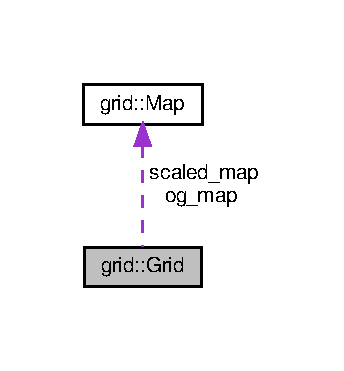
\includegraphics[width=165pt]{dc/d43/classgrid_1_1Grid__coll__graph}
\end{center}
\end{figure}
\subsection*{Public Member Functions}
\begin{DoxyCompactItemize}
\item 
\mbox{\Hypertarget{classgrid_1_1Grid_afcee115a9437842956e1efe9e202c302}\label{classgrid_1_1Grid_afcee115a9437842956e1efe9e202c302}} 
\hyperlink{classgrid_1_1Grid_afcee115a9437842956e1efe9e202c302}{Grid} ()
\begin{DoxyCompactList}\small\item\em Initialization to construct a grid in an empty 10x10 area. \end{DoxyCompactList}\item 
\hyperlink{classgrid_1_1Grid_a39cd30c1ee231fde7f5a3f228a326ac1}{Grid} (std\+::vector$<$ double $>$ xboundary, std\+::vector$<$ double $>$ yboundary)
\begin{DoxyCompactList}\small\item\em Initialization to construct a grid in an empty user defined area. \end{DoxyCompactList}\item 
\hyperlink{classgrid_1_1Grid_a3fd6c9bb56bc7ae63d6126312e001f23}{Grid} (std\+::vector$<$ std\+::vector$<$ rigid2d\+::\+Vector2D $>$$>$ polygon\+\_\+verticies, std\+::vector$<$ double $>$ xboundary, std\+::vector$<$ double $>$ yboundary)
\begin{DoxyCompactList}\small\item\em Initialization to construct a grid in a user defined area with obstacles. \end{DoxyCompactList}\item 
void \hyperlink{classgrid_1_1Grid_adcba03289a5d2de6e209b2a3ded5d5ac}{build\+\_\+grid} (double \hyperlink{classgrid_1_1Grid_acb1ca003a2aeafe6b554d9ac27b29109}{cell\+\_\+size}, unsigned int \hyperlink{classgrid_1_1Grid_a574ec32cb3346c1be8de79ccc38cd47b}{grid\+\_\+res}, double robot\+\_\+radius)
\begin{DoxyCompactList}\small\item\em Function to call all nessissary functions to build the grid. \end{DoxyCompactList}\item 
\mbox{\Hypertarget{classgrid_1_1Grid_a6620e51207bbd6ca60f868b120cb7e04}\label{classgrid_1_1Grid_a6620e51207bbd6ca60f868b120cb7e04}} 
void \hyperlink{classgrid_1_1Grid_a6620e51207bbd6ca60f868b120cb7e04}{generate\+\_\+centers\+\_\+graph} ()
\begin{DoxyCompactList}\small\item\em Function to generate an 8 neighbor connected graph structure based on grid cell center locations. \end{DoxyCompactList}\item 
std\+::vector$<$ int $>$ \hyperlink{classgrid_1_1Grid_adc9dda8d5d6bca20697790712b154cc1}{update\+\_\+grid} (std\+::vector$<$ std\+::pair$<$ rigid2d\+::\+Vector2D, signed char $>$$>$ points)
\begin{DoxyCompactList}\small\item\em Update the existing occupancy data with new information -\/ Note this does not update the stored \hyperlink{structgrid_1_1Map}{Map} variables, so calling \char`\"{}build\+\_\+grid\char`\"{} will revert the occ data based on the map used to create the grid. \end{DoxyCompactList}\item 
std\+::vector$<$ std\+::vector$<$ \hyperlink{structprm_1_1Node}{prm\+::\+Node} $>$ $>$ \hyperlink{classgrid_1_1Grid_a28e01687d0e3e922607e67b3d1d862b6}{get\+\_\+nodes} () const
\begin{DoxyCompactList}\small\item\em Retrive the nodes in a 2D vector in the shape of the grid. \end{DoxyCompactList}\item 
std\+::vector$<$ \hyperlink{structprm_1_1Node}{prm\+::\+Node} $>$ \hyperlink{classgrid_1_1Grid_adc6f8296117527ab16f352806e9dc1d6}{get\+\_\+nodes\+\_\+flatten} () const
\begin{DoxyCompactList}\small\item\em Retrive the nodes in row major order. \end{DoxyCompactList}\item 
std\+::vector$<$ \hyperlink{structprm_1_1Edge}{prm\+::\+Edge} $>$ \hyperlink{classgrid_1_1Grid_a22f08e25cb643d8813fc4332300185b7}{get\+\_\+edges} () const
\begin{DoxyCompactList}\small\item\em Retrive the unique edges in the graph. \end{DoxyCompactList}\item 
std\+::vector$<$ std\+::vector$<$ signed char $>$ $>$ \hyperlink{classgrid_1_1Grid_a9efaa72e19c8351e1979c6ac18517de4}{get\+\_\+grid} () const
\begin{DoxyCompactList}\small\item\em retrieve the built grid \end{DoxyCompactList}\item 
std\+::vector$<$ signed char $>$ \hyperlink{classgrid_1_1Grid_a7c05ad9408e0ff99e36a3196136f3bb7}{get\+\_\+grid\+\_\+flatten} () const
\begin{DoxyCompactList}\small\item\em convert the grid data into a in row major order with the first element corresponding to the lower left corner. \end{DoxyCompactList}\item 
std\+::vector$<$ int $>$ \hyperlink{classgrid_1_1Grid_ab5da2712457e615bb12ca6d5fc1f1b9d}{get\+\_\+grid\+\_\+dimensions} () const
\begin{DoxyCompactList}\small\item\em get the height and width of the grid \end{DoxyCompactList}\item 
rigid2d\+::\+Vector2D \hyperlink{classgrid_1_1Grid_a740d72189efbdf5595c3ddaacc8cdfc4}{grid\+\_\+to\+\_\+world} (rigid2d\+::\+Vector2D grid\+\_\+coord)
\begin{DoxyCompactList}\small\item\em convert from grid coordinates (integers) to world coordinates (meters) \end{DoxyCompactList}\item 
rigid2d\+::\+Vector2D \hyperlink{classgrid_1_1Grid_a9aeb33485b294ab4a07178359db6e3cf}{world\+\_\+to\+\_\+grid} (rigid2d\+::\+Vector2D world\+\_\+coord)
\begin{DoxyCompactList}\small\item\em convert from world coordinates to grid coordinates \end{DoxyCompactList}\end{DoxyCompactItemize}
\subsection*{Private Member Functions}
\begin{DoxyCompactItemize}
\item 
\mbox{\Hypertarget{classgrid_1_1Grid_af5dd6a34ea30b975c4e72304db4e6dc7}\label{classgrid_1_1Grid_af5dd6a34ea30b975c4e72304db4e6dc7}} 
void \hyperlink{classgrid_1_1Grid_af5dd6a34ea30b975c4e72304db4e6dc7}{grid\+\_\+resize} ()
\begin{DoxyCompactList}\small\item\em calculate the grid size based on the saved map and the grid resolution \end{DoxyCompactList}\item 
bool \hyperlink{classgrid_1_1Grid_a5b8625b7400116c5707c0465467a597d}{cell\+\_\+near\+\_\+boarder} (rigid2d\+::\+Vector2D center, double threshold)
\begin{DoxyCompactList}\small\item\em Determine if the cell center is within the buffer radius of the map boarder. \end{DoxyCompactList}\end{DoxyCompactItemize}
\subsection*{Private Attributes}
\begin{DoxyCompactItemize}
\item 
\mbox{\Hypertarget{classgrid_1_1Grid_a611cf14f1d75f0c77a7a5bcbc8fee6e0}\label{classgrid_1_1Grid_a611cf14f1d75f0c77a7a5bcbc8fee6e0}} 
\hyperlink{structgrid_1_1Map}{Map} \hyperlink{classgrid_1_1Grid_a611cf14f1d75f0c77a7a5bcbc8fee6e0}{og\+\_\+map}
\begin{DoxyCompactList}\small\item\em the map to initialize the grid with \end{DoxyCompactList}\item 
\mbox{\Hypertarget{classgrid_1_1Grid_ab990be4a53fd45a83df3f823f7098d56}\label{classgrid_1_1Grid_ab990be4a53fd45a83df3f823f7098d56}} 
\hyperlink{structgrid_1_1Map}{Map} \hyperlink{classgrid_1_1Grid_ab990be4a53fd45a83df3f823f7098d56}{scaled\+\_\+map}
\begin{DoxyCompactList}\small\item\em the scaled map based on the grid resolution \end{DoxyCompactList}\item 
\mbox{\Hypertarget{classgrid_1_1Grid_a375f27f536721667f4487b74982c154a}\label{classgrid_1_1Grid_a375f27f536721667f4487b74982c154a}} 
std\+::vector$<$ int $>$ \hyperlink{classgrid_1_1Grid_a375f27f536721667f4487b74982c154a}{grid\+\_\+dimensions}
\begin{DoxyCompactList}\small\item\em x, y \end{DoxyCompactList}\item 
\mbox{\Hypertarget{classgrid_1_1Grid_aae353051de1a48dd8f29e1889d71bf88}\label{classgrid_1_1Grid_aae353051de1a48dd8f29e1889d71bf88}} 
double \hyperlink{classgrid_1_1Grid_aae353051de1a48dd8f29e1889d71bf88}{buffer\+\_\+radius} = 0.\+0
\begin{DoxyCompactList}\small\item\em buffer distance to incorporate when detecting collisions \end{DoxyCompactList}\item 
\mbox{\Hypertarget{classgrid_1_1Grid_a574ec32cb3346c1be8de79ccc38cd47b}\label{classgrid_1_1Grid_a574ec32cb3346c1be8de79ccc38cd47b}} 
unsigned int \hyperlink{classgrid_1_1Grid_a574ec32cb3346c1be8de79ccc38cd47b}{grid\+\_\+res} = 1
\begin{DoxyCompactList}\small\item\em scale the cell size \end{DoxyCompactList}\item 
\mbox{\Hypertarget{classgrid_1_1Grid_acb1ca003a2aeafe6b554d9ac27b29109}\label{classgrid_1_1Grid_acb1ca003a2aeafe6b554d9ac27b29109}} 
double \hyperlink{classgrid_1_1Grid_acb1ca003a2aeafe6b554d9ac27b29109}{cell\+\_\+size} = 1.\+0
\begin{DoxyCompactList}\small\item\em meters per grid cell \end{DoxyCompactList}\item 
\mbox{\Hypertarget{classgrid_1_1Grid_a970c0980c3a662ddaddd9e457f799252}\label{classgrid_1_1Grid_a970c0980c3a662ddaddd9e457f799252}} 
std\+::vector$<$ std\+::vector$<$ \hyperlink{structprm_1_1Node}{prm\+::\+Node} $>$ $>$ \hyperlink{classgrid_1_1Grid_a970c0980c3a662ddaddd9e457f799252}{nodes}
\begin{DoxyCompactList}\small\item\em all nodes in the grid \end{DoxyCompactList}\item 
\mbox{\Hypertarget{classgrid_1_1Grid_a80fab4482c55128e29083184c234f197}\label{classgrid_1_1Grid_a80fab4482c55128e29083184c234f197}} 
std\+::vector$<$ \hyperlink{structprm_1_1Edge}{prm\+::\+Edge} $>$ \hyperlink{classgrid_1_1Grid_a80fab4482c55128e29083184c234f197}{all\+\_\+edges}
\begin{DoxyCompactList}\small\item\em all edges between the grid \end{DoxyCompactList}\item 
\mbox{\Hypertarget{classgrid_1_1Grid_a640e9d8f352ebb19ec2801229e5483e4}\label{classgrid_1_1Grid_a640e9d8f352ebb19ec2801229e5483e4}} 
std\+::vector$<$ std\+::vector$<$ signed char $>$ $>$ \hyperlink{classgrid_1_1Grid_a640e9d8f352ebb19ec2801229e5483e4}{occ\+\_\+data}
\begin{DoxyCompactList}\small\item\em occupancy grid data, 0 is free, 50 is buffer zone, 100 is occupied \end{DoxyCompactList}\end{DoxyCompactItemize}


\subsection{Detailed Description}
Class to create a \hyperlink{classgrid_1_1Grid}{Grid} overlay for provided \hyperlink{structgrid_1_1Map}{Map} information. 

\subsection{Constructor \& Destructor Documentation}
\mbox{\Hypertarget{classgrid_1_1Grid_a39cd30c1ee231fde7f5a3f228a326ac1}\label{classgrid_1_1Grid_a39cd30c1ee231fde7f5a3f228a326ac1}} 
\index{grid\+::\+Grid@{grid\+::\+Grid}!Grid@{Grid}}
\index{Grid@{Grid}!grid\+::\+Grid@{grid\+::\+Grid}}
\subsubsection{\texorpdfstring{Grid()}{Grid()}\hspace{0.1cm}{\footnotesize\ttfamily [1/2]}}
{\footnotesize\ttfamily grid\+::\+Grid\+::\+Grid (\begin{DoxyParamCaption}\item[{std\+::vector$<$ double $>$}]{xboundary,  }\item[{std\+::vector$<$ double $>$}]{yboundary }\end{DoxyParamCaption})}



Initialization to construct a grid in an empty user defined area. 


\begin{DoxyParams}{Parameters}
{\em xboundary} & a 2 element vector defining the map\textquotesingle{}s x bounds in integer coordinates \\
\hline
{\em yboundary} & a 2 element vector defining the map\textquotesingle{}s y bounds in integer coordinates \\
\hline
\end{DoxyParams}
\mbox{\Hypertarget{classgrid_1_1Grid_a3fd6c9bb56bc7ae63d6126312e001f23}\label{classgrid_1_1Grid_a3fd6c9bb56bc7ae63d6126312e001f23}} 
\index{grid\+::\+Grid@{grid\+::\+Grid}!Grid@{Grid}}
\index{Grid@{Grid}!grid\+::\+Grid@{grid\+::\+Grid}}
\subsubsection{\texorpdfstring{Grid()}{Grid()}\hspace{0.1cm}{\footnotesize\ttfamily [2/2]}}
{\footnotesize\ttfamily grid\+::\+Grid\+::\+Grid (\begin{DoxyParamCaption}\item[{std\+::vector$<$ std\+::vector$<$ rigid2d\+::\+Vector2D $>$$>$}]{polygon\+\_\+verticies,  }\item[{std\+::vector$<$ double $>$}]{xboundary,  }\item[{std\+::vector$<$ double $>$}]{yboundary }\end{DoxyParamCaption})}



Initialization to construct a grid in a user defined area with obstacles. 


\begin{DoxyParams}{Parameters}
{\em polygon\+\_\+verticies} & a vector of vectors defining the verticies of each obstacle in integer coordinates and in order going counter-\/clockwise \\
\hline
{\em xboundary} & a 2 element vector defining the map\textquotesingle{}s x bounds in integer coordinates \\
\hline
{\em yboundary} & a 2 element vector defining the map\textquotesingle{}s y bounds in integer coordinates \\
\hline
\end{DoxyParams}


\subsection{Member Function Documentation}
\mbox{\Hypertarget{classgrid_1_1Grid_adcba03289a5d2de6e209b2a3ded5d5ac}\label{classgrid_1_1Grid_adcba03289a5d2de6e209b2a3ded5d5ac}} 
\index{grid\+::\+Grid@{grid\+::\+Grid}!build\+\_\+grid@{build\+\_\+grid}}
\index{build\+\_\+grid@{build\+\_\+grid}!grid\+::\+Grid@{grid\+::\+Grid}}
\subsubsection{\texorpdfstring{build\+\_\+grid()}{build\_grid()}}
{\footnotesize\ttfamily void grid\+::\+Grid\+::build\+\_\+grid (\begin{DoxyParamCaption}\item[{double}]{cell\+\_\+size,  }\item[{unsigned int}]{grid\+\_\+res,  }\item[{double}]{robot\+\_\+radius }\end{DoxyParamCaption})}



Function to call all nessissary functions to build the grid. 


\begin{DoxyParams}{Parameters}
{\em cell\+\_\+size} & the desired distance the distance for the cell length/height in meters \\
\hline
{\em grid\+\_\+res} & scaling factor to create the occupancy grid with a finer resolution that the existing cell\+\_\+size. Use 1 to make the grid equal to the current cell size Use 2 to double the resolution. \\
\hline
{\em robot\+\_\+radius} & the radius to use as a buffer around the robot for collision detection \\
\hline
\end{DoxyParams}
\mbox{\Hypertarget{classgrid_1_1Grid_a5b8625b7400116c5707c0465467a597d}\label{classgrid_1_1Grid_a5b8625b7400116c5707c0465467a597d}} 
\index{grid\+::\+Grid@{grid\+::\+Grid}!cell\+\_\+near\+\_\+boarder@{cell\+\_\+near\+\_\+boarder}}
\index{cell\+\_\+near\+\_\+boarder@{cell\+\_\+near\+\_\+boarder}!grid\+::\+Grid@{grid\+::\+Grid}}
\subsubsection{\texorpdfstring{cell\+\_\+near\+\_\+boarder()}{cell\_near\_boarder()}}
{\footnotesize\ttfamily bool grid\+::\+Grid\+::cell\+\_\+near\+\_\+boarder (\begin{DoxyParamCaption}\item[{rigid2d\+::\+Vector2D}]{center,  }\item[{double}]{threshold }\end{DoxyParamCaption})\hspace{0.3cm}{\ttfamily [private]}}



Determine if the cell center is within the buffer radius of the map boarder. 


\begin{DoxyParams}{Parameters}
{\em center} & location of cell to check against \\
\hline
{\em threshold} & grid buffer distance \\
\hline
\end{DoxyParams}
\begin{DoxyReturn}{Returns}
True if the cell center is within the buffer\+\_\+radius 
\end{DoxyReturn}
\mbox{\Hypertarget{classgrid_1_1Grid_a22f08e25cb643d8813fc4332300185b7}\label{classgrid_1_1Grid_a22f08e25cb643d8813fc4332300185b7}} 
\index{grid\+::\+Grid@{grid\+::\+Grid}!get\+\_\+edges@{get\+\_\+edges}}
\index{get\+\_\+edges@{get\+\_\+edges}!grid\+::\+Grid@{grid\+::\+Grid}}
\subsubsection{\texorpdfstring{get\+\_\+edges()}{get\_edges()}}
{\footnotesize\ttfamily std\+::vector$<$ \hyperlink{structprm_1_1Edge}{prm\+::\+Edge} $>$ grid\+::\+Grid\+::get\+\_\+edges (\begin{DoxyParamCaption}{ }\end{DoxyParamCaption}) const}



Retrive the unique edges in the graph. 

\begin{DoxyReturn}{Returns}
all the unique edges 
\end{DoxyReturn}
\mbox{\Hypertarget{classgrid_1_1Grid_a9efaa72e19c8351e1979c6ac18517de4}\label{classgrid_1_1Grid_a9efaa72e19c8351e1979c6ac18517de4}} 
\index{grid\+::\+Grid@{grid\+::\+Grid}!get\+\_\+grid@{get\+\_\+grid}}
\index{get\+\_\+grid@{get\+\_\+grid}!grid\+::\+Grid@{grid\+::\+Grid}}
\subsubsection{\texorpdfstring{get\+\_\+grid()}{get\_grid()}}
{\footnotesize\ttfamily std\+::vector$<$ std\+::vector$<$ signed char $>$ $>$ grid\+::\+Grid\+::get\+\_\+grid (\begin{DoxyParamCaption}{ }\end{DoxyParamCaption}) const}



retrieve the built grid 

\begin{DoxyReturn}{Returns}
grid occupancy data as a vector of vectors. 
\end{DoxyReturn}
\mbox{\Hypertarget{classgrid_1_1Grid_ab5da2712457e615bb12ca6d5fc1f1b9d}\label{classgrid_1_1Grid_ab5da2712457e615bb12ca6d5fc1f1b9d}} 
\index{grid\+::\+Grid@{grid\+::\+Grid}!get\+\_\+grid\+\_\+dimensions@{get\+\_\+grid\+\_\+dimensions}}
\index{get\+\_\+grid\+\_\+dimensions@{get\+\_\+grid\+\_\+dimensions}!grid\+::\+Grid@{grid\+::\+Grid}}
\subsubsection{\texorpdfstring{get\+\_\+grid\+\_\+dimensions()}{get\_grid\_dimensions()}}
{\footnotesize\ttfamily std\+::vector$<$ int $>$ grid\+::\+Grid\+::get\+\_\+grid\+\_\+dimensions (\begin{DoxyParamCaption}{ }\end{DoxyParamCaption}) const}



get the height and width of the grid 

\begin{DoxyReturn}{Returns}
the grid dimensions in number of cells 
\end{DoxyReturn}
\mbox{\Hypertarget{classgrid_1_1Grid_a7c05ad9408e0ff99e36a3196136f3bb7}\label{classgrid_1_1Grid_a7c05ad9408e0ff99e36a3196136f3bb7}} 
\index{grid\+::\+Grid@{grid\+::\+Grid}!get\+\_\+grid\+\_\+flatten@{get\+\_\+grid\+\_\+flatten}}
\index{get\+\_\+grid\+\_\+flatten@{get\+\_\+grid\+\_\+flatten}!grid\+::\+Grid@{grid\+::\+Grid}}
\subsubsection{\texorpdfstring{get\+\_\+grid\+\_\+flatten()}{get\_grid\_flatten()}}
{\footnotesize\ttfamily std\+::vector$<$ signed char $>$ grid\+::\+Grid\+::get\+\_\+grid\+\_\+flatten (\begin{DoxyParamCaption}{ }\end{DoxyParamCaption}) const}



convert the grid data into a in row major order with the first element corresponding to the lower left corner. 

\begin{DoxyReturn}{Returns}
grid occupancy data in row major order 
\end{DoxyReturn}
\mbox{\Hypertarget{classgrid_1_1Grid_a28e01687d0e3e922607e67b3d1d862b6}\label{classgrid_1_1Grid_a28e01687d0e3e922607e67b3d1d862b6}} 
\index{grid\+::\+Grid@{grid\+::\+Grid}!get\+\_\+nodes@{get\+\_\+nodes}}
\index{get\+\_\+nodes@{get\+\_\+nodes}!grid\+::\+Grid@{grid\+::\+Grid}}
\subsubsection{\texorpdfstring{get\+\_\+nodes()}{get\_nodes()}}
{\footnotesize\ttfamily std\+::vector$<$ std\+::vector$<$ \hyperlink{structprm_1_1Node}{prm\+::\+Node} $>$ $>$ grid\+::\+Grid\+::get\+\_\+nodes (\begin{DoxyParamCaption}{ }\end{DoxyParamCaption}) const}



Retrive the nodes in a 2D vector in the shape of the grid. 

\begin{DoxyReturn}{Returns}
the nodes in a structure matching the grid 
\end{DoxyReturn}
\mbox{\Hypertarget{classgrid_1_1Grid_adc6f8296117527ab16f352806e9dc1d6}\label{classgrid_1_1Grid_adc6f8296117527ab16f352806e9dc1d6}} 
\index{grid\+::\+Grid@{grid\+::\+Grid}!get\+\_\+nodes\+\_\+flatten@{get\+\_\+nodes\+\_\+flatten}}
\index{get\+\_\+nodes\+\_\+flatten@{get\+\_\+nodes\+\_\+flatten}!grid\+::\+Grid@{grid\+::\+Grid}}
\subsubsection{\texorpdfstring{get\+\_\+nodes\+\_\+flatten()}{get\_nodes\_flatten()}}
{\footnotesize\ttfamily std\+::vector$<$ \hyperlink{structprm_1_1Node}{prm\+::\+Node} $>$ grid\+::\+Grid\+::get\+\_\+nodes\+\_\+flatten (\begin{DoxyParamCaption}{ }\end{DoxyParamCaption}) const}



Retrive the nodes in row major order. 

\begin{DoxyReturn}{Returns}
the nodes in a single row vector 
\end{DoxyReturn}
\mbox{\Hypertarget{classgrid_1_1Grid_a740d72189efbdf5595c3ddaacc8cdfc4}\label{classgrid_1_1Grid_a740d72189efbdf5595c3ddaacc8cdfc4}} 
\index{grid\+::\+Grid@{grid\+::\+Grid}!grid\+\_\+to\+\_\+world@{grid\+\_\+to\+\_\+world}}
\index{grid\+\_\+to\+\_\+world@{grid\+\_\+to\+\_\+world}!grid\+::\+Grid@{grid\+::\+Grid}}
\subsubsection{\texorpdfstring{grid\+\_\+to\+\_\+world()}{grid\_to\_world()}}
{\footnotesize\ttfamily rigid2d\+::\+Vector2D grid\+::\+Grid\+::grid\+\_\+to\+\_\+world (\begin{DoxyParamCaption}\item[{rigid2d\+::\+Vector2D}]{grid\+\_\+coord }\end{DoxyParamCaption})}



convert from grid coordinates (integers) to world coordinates (meters) 


\begin{DoxyParams}{Parameters}
{\em grid\+\_\+coord} & grid location to convert \\
\hline
\end{DoxyParams}
\begin{DoxyReturn}{Returns}
matching world coordinate 
\end{DoxyReturn}
\mbox{\Hypertarget{classgrid_1_1Grid_adc9dda8d5d6bca20697790712b154cc1}\label{classgrid_1_1Grid_adc9dda8d5d6bca20697790712b154cc1}} 
\index{grid\+::\+Grid@{grid\+::\+Grid}!update\+\_\+grid@{update\+\_\+grid}}
\index{update\+\_\+grid@{update\+\_\+grid}!grid\+::\+Grid@{grid\+::\+Grid}}
\subsubsection{\texorpdfstring{update\+\_\+grid()}{update\_grid()}}
{\footnotesize\ttfamily std\+::vector$<$ int $>$ grid\+::\+Grid\+::update\+\_\+grid (\begin{DoxyParamCaption}\item[{std\+::vector$<$ std\+::pair$<$ rigid2d\+::\+Vector2D, signed char $>$$>$}]{points }\end{DoxyParamCaption})}



Update the existing occupancy data with new information -\/ Note this does not update the stored \hyperlink{structgrid_1_1Map}{Map} variables, so calling \char`\"{}build\+\_\+grid\char`\"{} will revert the occ data based on the map used to create the grid. 


\begin{DoxyParams}{Parameters}
{\em points} & pairs of grid cell locations and new occupancy data to potentially update. \\
\hline
\end{DoxyParams}
\begin{DoxyReturn}{Returns}
a vector of boolean values\+: True if the new point info actually caused a change in the occupancy data from free to occupied, otherwise False. 
\end{DoxyReturn}
\mbox{\Hypertarget{classgrid_1_1Grid_a9aeb33485b294ab4a07178359db6e3cf}\label{classgrid_1_1Grid_a9aeb33485b294ab4a07178359db6e3cf}} 
\index{grid\+::\+Grid@{grid\+::\+Grid}!world\+\_\+to\+\_\+grid@{world\+\_\+to\+\_\+grid}}
\index{world\+\_\+to\+\_\+grid@{world\+\_\+to\+\_\+grid}!grid\+::\+Grid@{grid\+::\+Grid}}
\subsubsection{\texorpdfstring{world\+\_\+to\+\_\+grid()}{world\_to\_grid()}}
{\footnotesize\ttfamily rigid2d\+::\+Vector2D grid\+::\+Grid\+::world\+\_\+to\+\_\+grid (\begin{DoxyParamCaption}\item[{rigid2d\+::\+Vector2D}]{world\+\_\+coord }\end{DoxyParamCaption})}



convert from world coordinates to grid coordinates 


\begin{DoxyParams}{Parameters}
{\em world\+\_\+coord} & world location to convert \\
\hline
\end{DoxyParams}
\begin{DoxyReturn}{Returns}
matching grid coordinate 
\end{DoxyReturn}


The documentation for this class was generated from the following files\+:\begin{DoxyCompactItemize}
\item 
roadmap/include/roadmap/grid.\+hpp\item 
roadmap/src/roadmap/grid.\+cpp\end{DoxyCompactItemize}

\hypertarget{structgrid_1_1Map}{}\section{grid\+:\+:Map Struct Reference}
\label{structgrid_1_1Map}\index{grid\+::\+Map@{grid\+::\+Map}}


Contains information about a bound map.  




{\ttfamily \#include $<$grid.\+hpp$>$}

\subsection*{Public Member Functions}
\begin{DoxyCompactItemize}
\item 
\mbox{\Hypertarget{structgrid_1_1Map_aeedaf34b4dcd443691c796637cea73ce}\label{structgrid_1_1Map_aeedaf34b4dcd443691c796637cea73ce}} 
\hyperlink{structgrid_1_1Map_aeedaf34b4dcd443691c796637cea73ce}{Map} ()
\begin{DoxyCompactList}\small\item\em default constructor \end{DoxyCompactList}\item 
\hyperlink{structgrid_1_1Map_a124140efcef69cee1d90f5d81d01e8fa}{Map} (std\+::vector$<$ std\+::vector$<$ rigid2d\+::\+Vector2D $>$$>$ obs, std\+::vector$<$ double $>$ x, std\+::vector$<$ double $>$ y)
\begin{DoxyCompactList}\small\item\em Fully construct the map. \end{DoxyCompactList}\end{DoxyCompactItemize}
\subsection*{Public Attributes}
\begin{DoxyCompactItemize}
\item 
\mbox{\Hypertarget{structgrid_1_1Map_ab9f49bab16cb300a8de972a412c54375}\label{structgrid_1_1Map_ab9f49bab16cb300a8de972a412c54375}} 
std\+::vector$<$ std\+::vector$<$ rigid2d\+::\+Vector2D $>$ $>$ \hyperlink{structgrid_1_1Map_ab9f49bab16cb300a8de972a412c54375}{obstacles}
\begin{DoxyCompactList}\small\item\em obstacles in the map \end{DoxyCompactList}\item 
\mbox{\Hypertarget{structgrid_1_1Map_a44918e798d8fa1400ddf52bc52ce4c6f}\label{structgrid_1_1Map_a44918e798d8fa1400ddf52bc52ce4c6f}} 
std\+::vector$<$ double $>$ \hyperlink{structgrid_1_1Map_a44918e798d8fa1400ddf52bc52ce4c6f}{x\+\_\+bounds}
\begin{DoxyCompactList}\small\item\em x bounds of the map \end{DoxyCompactList}\item 
\mbox{\Hypertarget{structgrid_1_1Map_a5f51eeac70566244a15c1023e9f494fb}\label{structgrid_1_1Map_a5f51eeac70566244a15c1023e9f494fb}} 
std\+::vector$<$ double $>$ \hyperlink{structgrid_1_1Map_a5f51eeac70566244a15c1023e9f494fb}{y\+\_\+bounds}
\begin{DoxyCompactList}\small\item\em y bounds of the map \end{DoxyCompactList}\item 
\mbox{\Hypertarget{structgrid_1_1Map_a5ee687d67cff44b8e447b2b92603056b}\label{structgrid_1_1Map_a5ee687d67cff44b8e447b2b92603056b}} 
std\+::vector$<$ rigid2d\+::\+Vector2D $>$ \hyperlink{structgrid_1_1Map_a5ee687d67cff44b8e447b2b92603056b}{map\+\_\+vector}
\begin{DoxyCompactList}\small\item\em a vector of the map verticies in ccw order \end{DoxyCompactList}\end{DoxyCompactItemize}


\subsection{Detailed Description}
Contains information about a bound map. 

\subsection{Constructor \& Destructor Documentation}
\mbox{\Hypertarget{structgrid_1_1Map_a124140efcef69cee1d90f5d81d01e8fa}\label{structgrid_1_1Map_a124140efcef69cee1d90f5d81d01e8fa}} 
\index{grid\+::\+Map@{grid\+::\+Map}!Map@{Map}}
\index{Map@{Map}!grid\+::\+Map@{grid\+::\+Map}}
\subsubsection{\texorpdfstring{Map()}{Map()}}
{\footnotesize\ttfamily grid\+::\+Map\+::\+Map (\begin{DoxyParamCaption}\item[{std\+::vector$<$ std\+::vector$<$ rigid2d\+::\+Vector2D $>$$>$}]{obs,  }\item[{std\+::vector$<$ double $>$}]{x,  }\item[{std\+::vector$<$ double $>$}]{y }\end{DoxyParamCaption})}



Fully construct the map. 


\begin{DoxyParams}{Parameters}
{\em obs} & obstacles in the map \\
\hline
{\em x} & bounds of the map \\
\hline
{\em y} & bounds of the map \\
\hline
\end{DoxyParams}


The documentation for this struct was generated from the following files\+:\begin{DoxyCompactItemize}
\item 
roadmap/include/roadmap/grid.\+hpp\item 
roadmap/src/roadmap/grid.\+cpp\end{DoxyCompactItemize}

\hypertarget{structprm_1_1Node}{}\section{prm\+:\+:Node Struct Reference}
\label{structprm_1_1Node}\index{prm\+::\+Node@{prm\+::\+Node}}


A struct to define a node and interact with it.  




{\ttfamily \#include $<$prm.\+hpp$>$}

\subsection*{Public Member Functions}
\begin{DoxyCompactItemize}
\item 
bool \hyperlink{structprm_1_1Node_a166ab395f8fcb59f5d5367ca45f7bf51}{Is\+Connected} (int node\+\_\+id) const
\begin{DoxyCompactList}\small\item\em Determine if a node is connected to this one. \end{DoxyCompactList}\item 
bool \hyperlink{structprm_1_1Node_ad414f13a52664be229be3a594613fb45}{operator$<$} (const \hyperlink{structprm_1_1Node}{Node} \&rhs) const
\begin{DoxyCompactList}\small\item\em Compares the distance value of this node object and another. \end{DoxyCompactList}\end{DoxyCompactItemize}
\subsection*{Public Attributes}
\begin{DoxyCompactItemize}
\item 
\mbox{\Hypertarget{structprm_1_1Node_a538d85b9f504bdb39268bd3168fd9211}\label{structprm_1_1Node_a538d85b9f504bdb39268bd3168fd9211}} 
int \hyperlink{structprm_1_1Node_a538d85b9f504bdb39268bd3168fd9211}{id} = -\/1
\begin{DoxyCompactList}\small\item\em unique node ID \end{DoxyCompactList}\item 
\mbox{\Hypertarget{structprm_1_1Node_afcf2b1941863d8d9a60874a30b9d2938}\label{structprm_1_1Node_afcf2b1941863d8d9a60874a30b9d2938}} 
rigid2d\+::\+Vector2D \hyperlink{structprm_1_1Node_afcf2b1941863d8d9a60874a30b9d2938}{point}
\begin{DoxyCompactList}\small\item\em x,y location relative to the world \end{DoxyCompactList}\item 
\mbox{\Hypertarget{structprm_1_1Node_abf983b6e36e98f9caf0766b1e8c5500a}\label{structprm_1_1Node_abf983b6e36e98f9caf0766b1e8c5500a}} 
std\+::vector$<$ \hyperlink{structprm_1_1Edge}{Edge} $>$ \hyperlink{structprm_1_1Node_abf983b6e36e98f9caf0766b1e8c5500a}{edges}
\begin{DoxyCompactList}\small\item\em edges connecting to nearby nodes \end{DoxyCompactList}\item 
\mbox{\Hypertarget{structprm_1_1Node_a23d5570a4b85f7403399444e68d5aa52}\label{structprm_1_1Node_a23d5570a4b85f7403399444e68d5aa52}} 
std\+::unordered\+\_\+set$<$ int $>$ \hyperlink{structprm_1_1Node_a23d5570a4b85f7403399444e68d5aa52}{id\+\_\+set}
\begin{DoxyCompactList}\small\item\em nodes that should be connected \end{DoxyCompactList}\item 
\mbox{\Hypertarget{structprm_1_1Node_af137867e3fb1f9b0d3e43ef3fd8ddecd}\label{structprm_1_1Node_af137867e3fb1f9b0d3e43ef3fd8ddecd}} 
double \hyperlink{structprm_1_1Node_af137867e3fb1f9b0d3e43ef3fd8ddecd}{weight} = 0
\begin{DoxyCompactList}\small\item\em weight to determine if map is properly sampled \end{DoxyCompactList}\item 
\mbox{\Hypertarget{structprm_1_1Node_a4db5966bcf026eaa4f2cd07ea22bcb4f}\label{structprm_1_1Node_a4db5966bcf026eaa4f2cd07ea22bcb4f}} 
double \hyperlink{structprm_1_1Node_a4db5966bcf026eaa4f2cd07ea22bcb4f}{distance} =0
\begin{DoxyCompactList}\small\item\em the distance to a node, used to find k-\/nearest nodes \end{DoxyCompactList}\end{DoxyCompactItemize}


\subsection{Detailed Description}
A struct to define a node and interact with it. 

\subsection{Member Function Documentation}
\mbox{\Hypertarget{structprm_1_1Node_a166ab395f8fcb59f5d5367ca45f7bf51}\label{structprm_1_1Node_a166ab395f8fcb59f5d5367ca45f7bf51}} 
\index{prm\+::\+Node@{prm\+::\+Node}!Is\+Connected@{Is\+Connected}}
\index{Is\+Connected@{Is\+Connected}!prm\+::\+Node@{prm\+::\+Node}}
\subsubsection{\texorpdfstring{Is\+Connected()}{IsConnected()}}
{\footnotesize\ttfamily bool prm\+::\+Node\+::\+Is\+Connected (\begin{DoxyParamCaption}\item[{int}]{node\+\_\+id }\end{DoxyParamCaption}) const\hspace{0.3cm}{\ttfamily [inline]}}



Determine if a node is connected to this one. 


\begin{DoxyParams}{Parameters}
{\em node\+\_\+id} & ID to check for a connection \\
\hline
\end{DoxyParams}
\begin{DoxyReturn}{Returns}
True if a connection exists 
\end{DoxyReturn}
\mbox{\Hypertarget{structprm_1_1Node_ad414f13a52664be229be3a594613fb45}\label{structprm_1_1Node_ad414f13a52664be229be3a594613fb45}} 
\index{prm\+::\+Node@{prm\+::\+Node}!operator$<$@{operator$<$}}
\index{operator$<$@{operator$<$}!prm\+::\+Node@{prm\+::\+Node}}
\subsubsection{\texorpdfstring{operator$<$()}{operator<()}}
{\footnotesize\ttfamily bool prm\+::\+Node\+::operator$<$ (\begin{DoxyParamCaption}\item[{const \hyperlink{structprm_1_1Node}{Node} \&}]{rhs }\end{DoxyParamCaption}) const\hspace{0.3cm}{\ttfamily [inline]}}



Compares the distance value of this node object and another. 


\begin{DoxyParams}{Parameters}
{\em rhs} & pointer to another node object \\
\hline
\end{DoxyParams}
\begin{DoxyReturn}{Returns}
True if this node has a smaller distance 
\end{DoxyReturn}


The documentation for this struct was generated from the following file\+:\begin{DoxyCompactItemize}
\item 
roadmap/include/roadmap/\hyperlink{prm_8hpp}{prm.\+hpp}\end{DoxyCompactItemize}

\hypertarget{classprm_1_1RoadMap}{}\section{prm\+:\+:Road\+Map Class Reference}
\label{classprm_1_1RoadMap}\index{prm\+::\+Road\+Map@{prm\+::\+Road\+Map}}


A class to build a Probabilistic Road Maps based on provided Map information.  




{\ttfamily \#include $<$prm.\+hpp$>$}

\subsection*{Public Member Functions}
\begin{DoxyCompactItemize}
\item 
\mbox{\Hypertarget{classprm_1_1RoadMap_a877e89a3bd0b0df936181c94aaeacb59}\label{classprm_1_1RoadMap_a877e89a3bd0b0df936181c94aaeacb59}} 
\hyperlink{classprm_1_1RoadMap_a877e89a3bd0b0df936181c94aaeacb59}{Road\+Map} ()
\begin{DoxyCompactList}\small\item\em Initialization to construct a road map in an empty 10x10 area with 100 samples. \end{DoxyCompactList}\item 
\hyperlink{classprm_1_1RoadMap_a95a183725f0ee0f2b0ce2643aa1ed870}{Road\+Map} (std\+::vector$<$ double $>$ xboundary, std\+::vector$<$ double $>$ yboundary)
\begin{DoxyCompactList}\small\item\em Initialization to construct a road map in an empty user defined area. \end{DoxyCompactList}\item 
\hyperlink{classprm_1_1RoadMap_a1c44e6fa58b91b3b79bcf56e414dff44}{Road\+Map} (std\+::vector$<$ std\+::vector$<$ rigid2d\+::\+Vector2D $>$$>$ polygon\+\_\+verticies, std\+::vector$<$ double $>$ xboundary, std\+::vector$<$ double $>$ yboundary)
\begin{DoxyCompactList}\small\item\em Initialization to construct a road map in a user defined area with obstacles. \end{DoxyCompactList}\item 
void \hyperlink{classprm_1_1RoadMap_ab81f9c73d7539b570a2164369144c41f}{build\+\_\+map} (unsigned int samples, unsigned int k\+\_\+neighbors, double robot\+\_\+radius)
\begin{DoxyCompactList}\small\item\em Wrapper function to call all nessissary functions to build the P\+RM. \end{DoxyCompactList}\item 
std\+::vector$<$ \hyperlink{structprm_1_1Node}{Node} $>$ \hyperlink{classprm_1_1RoadMap_a9b8c5b9de9a678f1eb9a6ceaa9fd8bb0}{get\+\_\+nodes} () const
\begin{DoxyCompactList}\small\item\em Wrapper function to get the vector of nodes. \end{DoxyCompactList}\item 
std\+::vector$<$ \hyperlink{structprm_1_1Edge}{Edge} $>$ \hyperlink{classprm_1_1RoadMap_a9be7cb5cac090269e00125cc7dc0cfd6}{get\+\_\+edges} () const
\begin{DoxyCompactList}\small\item\em Wrapper function to get the vector of unique edges. \end{DoxyCompactList}\item 
bool \hyperlink{classprm_1_1RoadMap_a45f658affb0061cdfe9de396fdbd7268}{add\+\_\+node} (rigid2d\+::\+Vector2D point)
\begin{DoxyCompactList}\small\item\em Add a user defined node into the graph and create the edges. \end{DoxyCompactList}\end{DoxyCompactItemize}
\subsection*{Private Member Functions}
\begin{DoxyCompactItemize}
\item 
\mbox{\Hypertarget{classprm_1_1RoadMap_a0d91fcf77606b05494dfcae4a4945351}\label{classprm_1_1RoadMap_a0d91fcf77606b05494dfcae4a4945351}} 
void \hyperlink{classprm_1_1RoadMap_a0d91fcf77606b05494dfcae4a4945351}{sample\+\_\+config\+\_\+space} ()
\begin{DoxyCompactList}\small\item\em Randomly Sample the configuration space to retrieve a set of nodes for the roadmap. \end{DoxyCompactList}\item 
bool \hyperlink{classprm_1_1RoadMap_a73c24a16d78040b0d5f247f0cf181363}{node\+\_\+collisions} (rigid2d\+::\+Vector2D point)
\begin{DoxyCompactList}\small\item\em Determine if the node was sampled from an area inside an obstacle. \end{DoxyCompactList}\item 
void \hyperlink{classprm_1_1RoadMap_ad74dcd92a949ee573310790fa8b2cae1}{connect\+\_\+node} (\hyperlink{structprm_1_1Node}{Node} \&node)
\begin{DoxyCompactList}\small\item\em Find nodes that are near the provided reference and connect them if possible. \end{DoxyCompactList}\item 
\mbox{\Hypertarget{classprm_1_1RoadMap_a05eba7fbe20463c8b8a3463dfd141c30}\label{classprm_1_1RoadMap_a05eba7fbe20463c8b8a3463dfd141c30}} 
void \hyperlink{classprm_1_1RoadMap_a05eba7fbe20463c8b8a3463dfd141c30}{connect\+\_\+nodes} ()
\begin{DoxyCompactList}\small\item\em Find nodes that are near each other and connect them if possible. \end{DoxyCompactList}\item 
bool \hyperlink{classprm_1_1RoadMap_a518085e457cb12dcbe63cfa3cc5942be}{edge\+\_\+collisions} (\hyperlink{structprm_1_1Edge}{Edge} edge)
\begin{DoxyCompactList}\small\item\em wrapper for all of the edge collision methods \end{DoxyCompactList}\item 
std\+::vector$<$ std\+::reference\+\_\+wrapper$<$ \hyperlink{structprm_1_1Node}{Node} $>$ $>$ \hyperlink{classprm_1_1RoadMap_a88e8d2df6c41bdc5ee5df4debbd0324d}{nearest\+\_\+neighbors\+\_\+bf} (const \hyperlink{structprm_1_1Node}{Node} \&node)
\begin{DoxyCompactList}\small\item\em Brute force k-\/nearest search. \end{DoxyCompactList}\end{DoxyCompactItemize}
\subsection*{Private Attributes}
\begin{DoxyCompactItemize}
\item 
\mbox{\Hypertarget{classprm_1_1RoadMap_a5c4bd6165645faab938831e7890d077e}\label{classprm_1_1RoadMap_a5c4bd6165645faab938831e7890d077e}} 
std\+::vector$<$ std\+::vector$<$ rigid2d\+::\+Vector2D $>$ $>$ \hyperlink{classprm_1_1RoadMap_a5c4bd6165645faab938831e7890d077e}{obstacles}
\begin{DoxyCompactList}\small\item\em obstacles in the map \end{DoxyCompactList}\item 
\mbox{\Hypertarget{classprm_1_1RoadMap_a2ad1a820114f8832cde28136385ab2d4}\label{classprm_1_1RoadMap_a2ad1a820114f8832cde28136385ab2d4}} 
std\+::vector$<$ double $>$ \hyperlink{classprm_1_1RoadMap_a2ad1a820114f8832cde28136385ab2d4}{x\+\_\+bounds}
\begin{DoxyCompactList}\small\item\em x bounds of the map \end{DoxyCompactList}\item 
\mbox{\Hypertarget{classprm_1_1RoadMap_a74349888d97a0056b994aae47c0a4b07}\label{classprm_1_1RoadMap_a74349888d97a0056b994aae47c0a4b07}} 
std\+::vector$<$ double $>$ \hyperlink{classprm_1_1RoadMap_a74349888d97a0056b994aae47c0a4b07}{y\+\_\+bounds}
\begin{DoxyCompactList}\small\item\em y bounds of the map \end{DoxyCompactList}\item 
\mbox{\Hypertarget{classprm_1_1RoadMap_a5f13fcb691beb29fd4ef0b37b3c05c54}\label{classprm_1_1RoadMap_a5f13fcb691beb29fd4ef0b37b3c05c54}} 
std\+::vector$<$ \hyperlink{structprm_1_1Node}{Node} $>$ \hyperlink{classprm_1_1RoadMap_a5f13fcb691beb29fd4ef0b37b3c05c54}{nodes}
\begin{DoxyCompactList}\small\item\em all nodes in the road map \end{DoxyCompactList}\item 
\mbox{\Hypertarget{classprm_1_1RoadMap_a05410db39631cd38cd76aaaa72325895}\label{classprm_1_1RoadMap_a05410db39631cd38cd76aaaa72325895}} 
std\+::vector$<$ \hyperlink{structprm_1_1Edge}{Edge} $>$ \hyperlink{classprm_1_1RoadMap_a05410db39631cd38cd76aaaa72325895}{all\+\_\+edges}
\begin{DoxyCompactList}\small\item\em all edges in the road map \end{DoxyCompactList}\item 
\mbox{\Hypertarget{classprm_1_1RoadMap_a9caa7aa9541cfae82f0f848ab6accffb}\label{classprm_1_1RoadMap_a9caa7aa9541cfae82f0f848ab6accffb}} 
double \hyperlink{classprm_1_1RoadMap_a9caa7aa9541cfae82f0f848ab6accffb}{buffer\+\_\+radius} = 0
\begin{DoxyCompactList}\small\item\em buffer distance to incorporate when detecting collisions \end{DoxyCompactList}\item 
\mbox{\Hypertarget{classprm_1_1RoadMap_a03d4a7e9302f36c8e0a2bbeaeaba2c5e}\label{classprm_1_1RoadMap_a03d4a7e9302f36c8e0a2bbeaeaba2c5e}} 
unsigned int \hyperlink{classprm_1_1RoadMap_a03d4a7e9302f36c8e0a2bbeaeaba2c5e}{n} = 100
\begin{DoxyCompactList}\small\item\em number of nodes in the map \end{DoxyCompactList}\item 
\mbox{\Hypertarget{classprm_1_1RoadMap_ad761640fd616fead6e1943a6f493750b}\label{classprm_1_1RoadMap_ad761640fd616fead6e1943a6f493750b}} 
unsigned int \hyperlink{classprm_1_1RoadMap_ad761640fd616fead6e1943a6f493750b}{k} = 10
\begin{DoxyCompactList}\small\item\em number of nearest neighbors to find \end{DoxyCompactList}\item 
\mbox{\Hypertarget{classprm_1_1RoadMap_ad5b8d4f3c026cc9e4b5bd8dff74a107e}\label{classprm_1_1RoadMap_ad5b8d4f3c026cc9e4b5bd8dff74a107e}} 
unsigned int \hyperlink{classprm_1_1RoadMap_ad5b8d4f3c026cc9e4b5bd8dff74a107e}{edge\+\_\+cnt} = 0
\begin{DoxyCompactList}\small\item\em number of edges in the graph \end{DoxyCompactList}\item 
\mbox{\Hypertarget{classprm_1_1RoadMap_a805350e531aa3e4992d941c399461842}\label{classprm_1_1RoadMap_a805350e531aa3e4992d941c399461842}} 
unsigned int \hyperlink{classprm_1_1RoadMap_a805350e531aa3e4992d941c399461842}{node\+\_\+cnt} = 0
\begin{DoxyCompactList}\small\item\em number of nodes in the graph \end{DoxyCompactList}\end{DoxyCompactItemize}


\subsection{Detailed Description}
A class to build a Probabilistic Road Maps based on provided Map information. 

\subsection{Constructor \& Destructor Documentation}
\mbox{\Hypertarget{classprm_1_1RoadMap_a95a183725f0ee0f2b0ce2643aa1ed870}\label{classprm_1_1RoadMap_a95a183725f0ee0f2b0ce2643aa1ed870}} 
\index{prm\+::\+Road\+Map@{prm\+::\+Road\+Map}!Road\+Map@{Road\+Map}}
\index{Road\+Map@{Road\+Map}!prm\+::\+Road\+Map@{prm\+::\+Road\+Map}}
\subsubsection{\texorpdfstring{Road\+Map()}{RoadMap()}\hspace{0.1cm}{\footnotesize\ttfamily [1/2]}}
{\footnotesize\ttfamily prm\+::\+Road\+Map\+::\+Road\+Map (\begin{DoxyParamCaption}\item[{std\+::vector$<$ double $>$}]{xboundary,  }\item[{std\+::vector$<$ double $>$}]{yboundary }\end{DoxyParamCaption})}



Initialization to construct a road map in an empty user defined area. 


\begin{DoxyParams}{Parameters}
{\em xboundary} & a 2 element vector defining the map\textquotesingle{}s x bounds \\
\hline
{\em yboundary} & a 2 element vector defining the map\textquotesingle{}s y bounds \\
\hline
\end{DoxyParams}
\mbox{\Hypertarget{classprm_1_1RoadMap_a1c44e6fa58b91b3b79bcf56e414dff44}\label{classprm_1_1RoadMap_a1c44e6fa58b91b3b79bcf56e414dff44}} 
\index{prm\+::\+Road\+Map@{prm\+::\+Road\+Map}!Road\+Map@{Road\+Map}}
\index{Road\+Map@{Road\+Map}!prm\+::\+Road\+Map@{prm\+::\+Road\+Map}}
\subsubsection{\texorpdfstring{Road\+Map()}{RoadMap()}\hspace{0.1cm}{\footnotesize\ttfamily [2/2]}}
{\footnotesize\ttfamily prm\+::\+Road\+Map\+::\+Road\+Map (\begin{DoxyParamCaption}\item[{std\+::vector$<$ std\+::vector$<$ rigid2d\+::\+Vector2D $>$$>$}]{polygon\+\_\+verticies,  }\item[{std\+::vector$<$ double $>$}]{xboundary,  }\item[{std\+::vector$<$ double $>$}]{yboundary }\end{DoxyParamCaption})}



Initialization to construct a road map in a user defined area with obstacles. 


\begin{DoxyParams}{Parameters}
{\em polygon\+\_\+verticies} & a vector of vectors defining the verticies of each obstacle in order going counter-\/clockwise \\
\hline
{\em xboundary} & a 2 element vector defining the map\textquotesingle{}s x bounds \\
\hline
{\em yboundary} & a 2 element vector defining the map\textquotesingle{}s y bounds \\
\hline
\end{DoxyParams}


\subsection{Member Function Documentation}
\mbox{\Hypertarget{classprm_1_1RoadMap_a45f658affb0061cdfe9de396fdbd7268}\label{classprm_1_1RoadMap_a45f658affb0061cdfe9de396fdbd7268}} 
\index{prm\+::\+Road\+Map@{prm\+::\+Road\+Map}!add\+\_\+node@{add\+\_\+node}}
\index{add\+\_\+node@{add\+\_\+node}!prm\+::\+Road\+Map@{prm\+::\+Road\+Map}}
\subsubsection{\texorpdfstring{add\+\_\+node()}{add\_node()}}
{\footnotesize\ttfamily bool prm\+::\+Road\+Map\+::add\+\_\+node (\begin{DoxyParamCaption}\item[{rigid2d\+::\+Vector2D}]{point }\end{DoxyParamCaption})}



Add a user defined node into the graph and create the edges. 


\begin{DoxyParams}{Parameters}
{\em point} & the x,y coordinates for the new node \\
\hline
\end{DoxyParams}
\begin{DoxyReturn}{Returns}
True if the node was successfully added 
\end{DoxyReturn}
\mbox{\Hypertarget{classprm_1_1RoadMap_ab81f9c73d7539b570a2164369144c41f}\label{classprm_1_1RoadMap_ab81f9c73d7539b570a2164369144c41f}} 
\index{prm\+::\+Road\+Map@{prm\+::\+Road\+Map}!build\+\_\+map@{build\+\_\+map}}
\index{build\+\_\+map@{build\+\_\+map}!prm\+::\+Road\+Map@{prm\+::\+Road\+Map}}
\subsubsection{\texorpdfstring{build\+\_\+map()}{build\_map()}}
{\footnotesize\ttfamily void prm\+::\+Road\+Map\+::build\+\_\+map (\begin{DoxyParamCaption}\item[{unsigned int}]{samples,  }\item[{unsigned int}]{k\+\_\+neighbors,  }\item[{double}]{robot\+\_\+radius }\end{DoxyParamCaption})}



Wrapper function to call all nessissary functions to build the P\+RM. 


\begin{DoxyParams}{Parameters}
{\em samples} & the number of nodes for the road map \\
\hline
{\em k\+\_\+neighbors} & the amount of neighbors to try and create an edge to \\
\hline
{\em robot\+\_\+radius} & the radius to use as a buffer around the robot for collision detection \\
\hline
\end{DoxyParams}
\mbox{\Hypertarget{classprm_1_1RoadMap_ad74dcd92a949ee573310790fa8b2cae1}\label{classprm_1_1RoadMap_ad74dcd92a949ee573310790fa8b2cae1}} 
\index{prm\+::\+Road\+Map@{prm\+::\+Road\+Map}!connect\+\_\+node@{connect\+\_\+node}}
\index{connect\+\_\+node@{connect\+\_\+node}!prm\+::\+Road\+Map@{prm\+::\+Road\+Map}}
\subsubsection{\texorpdfstring{connect\+\_\+node()}{connect\_node()}}
{\footnotesize\ttfamily void prm\+::\+Road\+Map\+::connect\+\_\+node (\begin{DoxyParamCaption}\item[{\hyperlink{structprm_1_1Node}{Node} \&}]{node }\end{DoxyParamCaption})\hspace{0.3cm}{\ttfamily [private]}}



Find nodes that are near the provided reference and connect them if possible. 


\begin{DoxyParams}{Parameters}
{\em node} & reference to a node \\
\hline
\end{DoxyParams}
\mbox{\Hypertarget{classprm_1_1RoadMap_a518085e457cb12dcbe63cfa3cc5942be}\label{classprm_1_1RoadMap_a518085e457cb12dcbe63cfa3cc5942be}} 
\index{prm\+::\+Road\+Map@{prm\+::\+Road\+Map}!edge\+\_\+collisions@{edge\+\_\+collisions}}
\index{edge\+\_\+collisions@{edge\+\_\+collisions}!prm\+::\+Road\+Map@{prm\+::\+Road\+Map}}
\subsubsection{\texorpdfstring{edge\+\_\+collisions()}{edge\_collisions()}}
{\footnotesize\ttfamily bool prm\+::\+Road\+Map\+::edge\+\_\+collisions (\begin{DoxyParamCaption}\item[{\hyperlink{structprm_1_1Edge}{Edge}}]{edge }\end{DoxyParamCaption})\hspace{0.3cm}{\ttfamily [private]}}



wrapper for all of the edge collision methods 


\begin{DoxyParams}{Parameters}
{\em edge} & the edge to compare against all polygons \\
\hline
\end{DoxyParams}
\begin{DoxyReturn}{Returns}
true if the edge is valid 
\end{DoxyReturn}
\mbox{\Hypertarget{classprm_1_1RoadMap_a9be7cb5cac090269e00125cc7dc0cfd6}\label{classprm_1_1RoadMap_a9be7cb5cac090269e00125cc7dc0cfd6}} 
\index{prm\+::\+Road\+Map@{prm\+::\+Road\+Map}!get\+\_\+edges@{get\+\_\+edges}}
\index{get\+\_\+edges@{get\+\_\+edges}!prm\+::\+Road\+Map@{prm\+::\+Road\+Map}}
\subsubsection{\texorpdfstring{get\+\_\+edges()}{get\_edges()}}
{\footnotesize\ttfamily std\+::vector$<$ \hyperlink{structprm_1_1Edge}{Edge} $>$ prm\+::\+Road\+Map\+::get\+\_\+edges (\begin{DoxyParamCaption}{ }\end{DoxyParamCaption}) const}



Wrapper function to get the vector of unique edges. 

\begin{DoxyReturn}{Returns}
the full edge vector 
\end{DoxyReturn}
\mbox{\Hypertarget{classprm_1_1RoadMap_a9b8c5b9de9a678f1eb9a6ceaa9fd8bb0}\label{classprm_1_1RoadMap_a9b8c5b9de9a678f1eb9a6ceaa9fd8bb0}} 
\index{prm\+::\+Road\+Map@{prm\+::\+Road\+Map}!get\+\_\+nodes@{get\+\_\+nodes}}
\index{get\+\_\+nodes@{get\+\_\+nodes}!prm\+::\+Road\+Map@{prm\+::\+Road\+Map}}
\subsubsection{\texorpdfstring{get\+\_\+nodes()}{get\_nodes()}}
{\footnotesize\ttfamily std\+::vector$<$ \hyperlink{structprm_1_1Node}{Node} $>$ prm\+::\+Road\+Map\+::get\+\_\+nodes (\begin{DoxyParamCaption}{ }\end{DoxyParamCaption}) const}



Wrapper function to get the vector of nodes. 

\begin{DoxyReturn}{Returns}
the full node vector 
\end{DoxyReturn}
\mbox{\Hypertarget{classprm_1_1RoadMap_a88e8d2df6c41bdc5ee5df4debbd0324d}\label{classprm_1_1RoadMap_a88e8d2df6c41bdc5ee5df4debbd0324d}} 
\index{prm\+::\+Road\+Map@{prm\+::\+Road\+Map}!nearest\+\_\+neighbors\+\_\+bf@{nearest\+\_\+neighbors\+\_\+bf}}
\index{nearest\+\_\+neighbors\+\_\+bf@{nearest\+\_\+neighbors\+\_\+bf}!prm\+::\+Road\+Map@{prm\+::\+Road\+Map}}
\subsubsection{\texorpdfstring{nearest\+\_\+neighbors\+\_\+bf()}{nearest\_neighbors\_bf()}}
{\footnotesize\ttfamily std\+::vector$<$ std\+::reference\+\_\+wrapper$<$ \hyperlink{structprm_1_1Node}{Node} $>$ $>$ prm\+::\+Road\+Map\+::nearest\+\_\+neighbors\+\_\+bf (\begin{DoxyParamCaption}\item[{const \hyperlink{structprm_1_1Node}{Node} \&}]{node }\end{DoxyParamCaption})\hspace{0.3cm}{\ttfamily [private]}}



Brute force k-\/nearest search. 


\begin{DoxyParams}{Parameters}
{\em reference} & to a node object to base the search on \\
\hline
\end{DoxyParams}
\begin{DoxyReturn}{Returns}
a vector of references the k-\/nearest nodes to the input node 
\end{DoxyReturn}
\mbox{\Hypertarget{classprm_1_1RoadMap_a73c24a16d78040b0d5f247f0cf181363}\label{classprm_1_1RoadMap_a73c24a16d78040b0d5f247f0cf181363}} 
\index{prm\+::\+Road\+Map@{prm\+::\+Road\+Map}!node\+\_\+collisions@{node\+\_\+collisions}}
\index{node\+\_\+collisions@{node\+\_\+collisions}!prm\+::\+Road\+Map@{prm\+::\+Road\+Map}}
\subsubsection{\texorpdfstring{node\+\_\+collisions()}{node\_collisions()}}
{\footnotesize\ttfamily bool prm\+::\+Road\+Map\+::node\+\_\+collisions (\begin{DoxyParamCaption}\item[{rigid2d\+::\+Vector2D}]{point }\end{DoxyParamCaption})\hspace{0.3cm}{\ttfamily [private]}}



Determine if the node was sampled from an area inside an obstacle. 


\begin{DoxyParams}{Parameters}
{\em point} & the configuration of a new potential node \\
\hline
\end{DoxyParams}
\begin{DoxyReturn}{Returns}
true if the node is valid 
\end{DoxyReturn}


The documentation for this class was generated from the following files\+:\begin{DoxyCompactItemize}
\item 
roadmap/include/roadmap/prm.\+hpp\item 
roadmap/src/roadmap/prm.\+cpp\end{DoxyCompactItemize}

\chapter{File Documentation}
\hypertarget{collision_8hpp}{}\section{roadmap/include/roadmap/collision.hpp File Reference}
\label{collision_8hpp}\index{roadmap/include/roadmap/collision.\+hpp@{roadmap/include/roadmap/collision.\+hpp}}


A library containing functions to detect various types of collisions.  


{\ttfamily \#include \char`\"{}rigid2d/rigid2d.\+hpp\char`\"{}}\newline
Include dependency graph for collision.\+hpp\+:\nopagebreak
\begin{figure}[H]
\begin{center}
\leavevmode
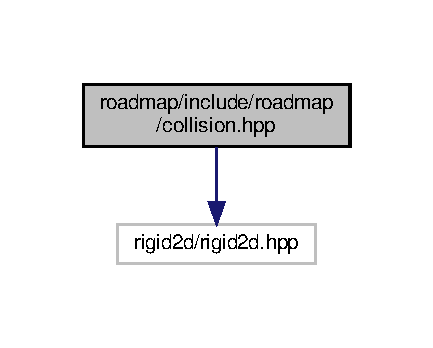
\includegraphics[width=208pt]{d9/d9b/collision_8hpp__incl}
\end{center}
\end{figure}
This graph shows which files directly or indirectly include this file\+:\nopagebreak
\begin{figure}[H]
\begin{center}
\leavevmode
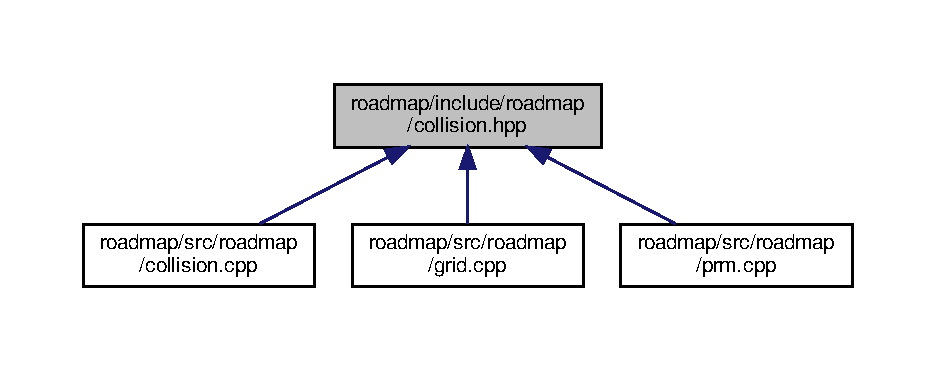
\includegraphics[width=350pt]{d2/d5b/collision_8hpp__dep__incl}
\end{center}
\end{figure}
\subsection*{Classes}
\begin{DoxyCompactItemize}
\item 
struct \hyperlink{structcollision_1_1DistRes}{collision\+::\+Dist\+Res}
\begin{DoxyCompactList}\small\item\em Used to return information from the point to line distance function. \end{DoxyCompactList}\end{DoxyCompactItemize}
\subsection*{Functions}
\begin{DoxyCompactItemize}
\item 
bool \hyperlink{collision_8hpp_aabf5aea7b02c454140c9bb242ca6e944}{collision\+::point\+\_\+to\+\_\+line\+\_\+distance} (rigid2d\+::\+Vector2D line\+\_\+start, rigid2d\+::\+Vector2D line\+\_\+end, rigid2d\+::\+Vector2D point, double threshold)
\begin{DoxyCompactList}\small\item\em Determine if a point is within a certain distance to a line. \end{DoxyCompactList}\item 
Dist\+Res \hyperlink{collision_8hpp_a7ac784d9a63acc273489e7e61c45416a}{collision\+::point\+\_\+to\+\_\+line\+\_\+distance} (rigid2d\+::\+Vector2D line\+\_\+start, rigid2d\+::\+Vector2D line\+\_\+end, rigid2d\+::\+Vector2D point)
\begin{DoxyCompactList}\small\item\em Calculate the minimum distance to a line segment. \end{DoxyCompactList}\item 
std\+::vector$<$ bool $>$ \hyperlink{collision_8hpp_af534ea532917e73ac2b28ca11c6cdf9f}{collision\+::point\+\_\+inside\+\_\+convex} (rigid2d\+::\+Vector2D point, std\+::vector$<$ rigid2d\+::\+Vector2D $>$ polygon, double buffer\+\_\+radius)
\begin{DoxyCompactList}\small\item\em Determine if a point is inside of a convex polygon, the points must be provided in order either cw or ccw. This function will account for connected the last vertex to the first vertex by appending the first vertex to the back of the vector. \end{DoxyCompactList}\item 
bool \hyperlink{collision_8hpp_a70c9083464a3dd4bc7c32dabe857e331}{collision\+::line\+\_\+shape\+\_\+intersection} (rigid2d\+::\+Vector2D line\+\_\+start, rigid2d\+::\+Vector2D line\+\_\+end, std\+::vector$<$ rigid2d\+::\+Vector2D $>$ polygon)
\begin{DoxyCompactList}\small\item\em Determine if a line segment intersects a convex polygon. \end{DoxyCompactList}\item 
bool \hyperlink{collision_8hpp_abf9b390bd1d767fe39f7d4806fae6b62}{collision\+::line\+\_\+shape\+\_\+intersection} (rigid2d\+::\+Vector2D line\+\_\+start, rigid2d\+::\+Vector2D line\+\_\+end, std\+::vector$<$ rigid2d\+::\+Vector2D $>$ polygon, double buffer\+\_\+radius)
\begin{DoxyCompactList}\small\item\em Determine if a line segment intersects a convex polygon or comes within a certain distance of it. This assumes the line start and end points are known to be outside of the buffer area of the polygon. \end{DoxyCompactList}\end{DoxyCompactItemize}


\subsection{Detailed Description}
A library containing functions to detect various types of collisions. 



\subsection{Function Documentation}
\mbox{\Hypertarget{collision_8hpp_file_a70c9083464a3dd4bc7c32dabe857e331}\label{collision_8hpp_file_a70c9083464a3dd4bc7c32dabe857e331}} 
\index{collision.\+hpp@{collision.\+hpp}!line\+\_\+shape\+\_\+intersection@{line\+\_\+shape\+\_\+intersection}}
\index{line\+\_\+shape\+\_\+intersection@{line\+\_\+shape\+\_\+intersection}!collision.\+hpp@{collision.\+hpp}}
\subsubsection{\texorpdfstring{line\+\_\+shape\+\_\+intersection()}{line\_shape\_intersection()}\hspace{0.1cm}{\footnotesize\ttfamily [1/2]}}
{\footnotesize\ttfamily bool collision\+::line\+\_\+shape\+\_\+intersection (\begin{DoxyParamCaption}\item[{rigid2d\+::\+Vector2D}]{line\+\_\+start,  }\item[{rigid2d\+::\+Vector2D}]{line\+\_\+end,  }\item[{std\+::vector$<$ rigid2d\+::\+Vector2D $>$}]{polygon }\end{DoxyParamCaption})}



Determine if a line segment intersects a convex polygon. 


\begin{DoxyParams}{Parameters}
{\em line\+\_\+start} & the point of the beginning of the line segment \\
\hline
{\em line\+\_\+end} & the point of the end of the line segment \\
\hline
{\em polygon} & a vector of verticies that define the polygon in ccw order \\
\hline
\end{DoxyParams}
\begin{DoxyReturn}{Returns}
True if there is an intersection between the line segment and polygon 
\end{DoxyReturn}
\mbox{\Hypertarget{collision_8hpp_file_abf9b390bd1d767fe39f7d4806fae6b62}\label{collision_8hpp_file_abf9b390bd1d767fe39f7d4806fae6b62}} 
\index{collision.\+hpp@{collision.\+hpp}!line\+\_\+shape\+\_\+intersection@{line\+\_\+shape\+\_\+intersection}}
\index{line\+\_\+shape\+\_\+intersection@{line\+\_\+shape\+\_\+intersection}!collision.\+hpp@{collision.\+hpp}}
\subsubsection{\texorpdfstring{line\+\_\+shape\+\_\+intersection()}{line\_shape\_intersection()}\hspace{0.1cm}{\footnotesize\ttfamily [2/2]}}
{\footnotesize\ttfamily bool collision\+::line\+\_\+shape\+\_\+intersection (\begin{DoxyParamCaption}\item[{rigid2d\+::\+Vector2D}]{line\+\_\+start,  }\item[{rigid2d\+::\+Vector2D}]{line\+\_\+end,  }\item[{std\+::vector$<$ rigid2d\+::\+Vector2D $>$}]{polygon,  }\item[{double}]{buffer\+\_\+radius }\end{DoxyParamCaption})}



Determine if a line segment intersects a convex polygon or comes within a certain distance of it. This assumes the line start and end points are known to be outside of the buffer area of the polygon. 


\begin{DoxyParams}{Parameters}
{\em line\+\_\+start} & the point of the beginning of the line segment \\
\hline
{\em line\+\_\+end} & the point of the end of the line segment \\
\hline
{\em polygon} & a vector of verticies that define the polygon in ccw order \\
\hline
{\em buffer\+\_\+radius} & a buffer distance to incorporate to the polygon boundary \\
\hline
\end{DoxyParams}
\begin{DoxyReturn}{Returns}
True if there is an intersection between the line segment and polygon or if the minimum distance to the line and shape is less than the buffer radius 
\end{DoxyReturn}
\mbox{\Hypertarget{collision_8hpp_file_af534ea532917e73ac2b28ca11c6cdf9f}\label{collision_8hpp_file_af534ea532917e73ac2b28ca11c6cdf9f}} 
\index{collision.\+hpp@{collision.\+hpp}!point\+\_\+inside\+\_\+convex@{point\+\_\+inside\+\_\+convex}}
\index{point\+\_\+inside\+\_\+convex@{point\+\_\+inside\+\_\+convex}!collision.\+hpp@{collision.\+hpp}}
\subsubsection{\texorpdfstring{point\+\_\+inside\+\_\+convex()}{point\_inside\_convex()}}
{\footnotesize\ttfamily std\+::vector$<$ bool $>$ collision\+::point\+\_\+inside\+\_\+convex (\begin{DoxyParamCaption}\item[{rigid2d\+::\+Vector2D}]{point,  }\item[{std\+::vector$<$ rigid2d\+::\+Vector2D $>$}]{polygon,  }\item[{double}]{buffer\+\_\+radius }\end{DoxyParamCaption})}



Determine if a point is inside of a convex polygon, the points must be provided in order either cw or ccw. This function will account for connected the last vertex to the first vertex by appending the first vertex to the back of the vector. 


\begin{DoxyParams}{Parameters}
{\em point} & the point to analyze \\
\hline
{\em polygon} & a vector of verticies that define the polygon in order, either cw or ccw. \\
\hline
{\em buffer\+\_\+radius} & a buffer distance to incorporate to the polygon boundary \\
\hline
\end{DoxyParams}
\begin{DoxyReturn}{Returns}
a 2 element vector, first element is true if there is a collision, second element describes the cause\+: True for inside the shape, False for outside the shape but in the buffer zone. 
\end{DoxyReturn}
\mbox{\Hypertarget{collision_8hpp_file_aabf5aea7b02c454140c9bb242ca6e944}\label{collision_8hpp_file_aabf5aea7b02c454140c9bb242ca6e944}} 
\index{collision.\+hpp@{collision.\+hpp}!point\+\_\+to\+\_\+line\+\_\+distance@{point\+\_\+to\+\_\+line\+\_\+distance}}
\index{point\+\_\+to\+\_\+line\+\_\+distance@{point\+\_\+to\+\_\+line\+\_\+distance}!collision.\+hpp@{collision.\+hpp}}
\subsubsection{\texorpdfstring{point\+\_\+to\+\_\+line\+\_\+distance()}{point\_to\_line\_distance()}\hspace{0.1cm}{\footnotesize\ttfamily [1/2]}}
{\footnotesize\ttfamily bool collision\+::point\+\_\+to\+\_\+line\+\_\+distance (\begin{DoxyParamCaption}\item[{rigid2d\+::\+Vector2D}]{line\+\_\+start,  }\item[{rigid2d\+::\+Vector2D}]{line\+\_\+end,  }\item[{rigid2d\+::\+Vector2D}]{point,  }\item[{double}]{threshold }\end{DoxyParamCaption})}



Determine if a point is within a certain distance to a line. 


\begin{DoxyParams}{Parameters}
{\em line\+\_\+start} & the point of the beginning of the line segment \\
\hline
{\em line\+\_\+end} & the point of the end of the line segment \\
\hline
{\em point} & the point to calculate the distance for \\
\hline
{\em threshold} & the distance threshold to compare against \\
\hline
\end{DoxyParams}
\begin{DoxyReturn}{Returns}
True if the distance between the point and the line is L\+E\+SS T\+H\+AN the provided threshold 
\end{DoxyReturn}
\mbox{\Hypertarget{collision_8hpp_file_a7ac784d9a63acc273489e7e61c45416a}\label{collision_8hpp_file_a7ac784d9a63acc273489e7e61c45416a}} 
\index{collision.\+hpp@{collision.\+hpp}!point\+\_\+to\+\_\+line\+\_\+distance@{point\+\_\+to\+\_\+line\+\_\+distance}}
\index{point\+\_\+to\+\_\+line\+\_\+distance@{point\+\_\+to\+\_\+line\+\_\+distance}!collision.\+hpp@{collision.\+hpp}}
\subsubsection{\texorpdfstring{point\+\_\+to\+\_\+line\+\_\+distance()}{point\_to\_line\_distance()}\hspace{0.1cm}{\footnotesize\ttfamily [2/2]}}
{\footnotesize\ttfamily Dist\+Res collision\+::point\+\_\+to\+\_\+line\+\_\+distance (\begin{DoxyParamCaption}\item[{rigid2d\+::\+Vector2D}]{line\+\_\+start,  }\item[{rigid2d\+::\+Vector2D}]{line\+\_\+end,  }\item[{rigid2d\+::\+Vector2D}]{point }\end{DoxyParamCaption})}



Calculate the minimum distance to a line segment. 


\begin{DoxyParams}{Parameters}
{\em line\+\_\+start} & the point of the beginning of the line segment \\
\hline
{\em line\+\_\+end} & the point of the end of the line segment \\
\hline
{\em point} & the point to calculate the distance for \\
\hline
\end{DoxyParams}
\begin{DoxyReturn}{Returns}
The shortest distance between the point and the line if the point is within the line segment or the minimum between the distances to the line\+\_\+start or line\+\_\+end 
\end{DoxyReturn}

\hypertarget{grid_8hpp}{}\section{roadmap/include/roadmap/grid.hpp File Reference}
\label{grid_8hpp}\index{roadmap/include/roadmap/grid.\+hpp@{roadmap/include/roadmap/grid.\+hpp}}


A library for building an occupancy grid.  


{\ttfamily \#include $<$vector$>$}\newline
{\ttfamily \#include $<$unordered\+\_\+set$>$}\newline
{\ttfamily \#include \char`\"{}rigid2d/rigid2d.\+hpp\char`\"{}}\newline
Include dependency graph for grid.\+hpp\+:\nopagebreak
\begin{figure}[H]
\begin{center}
\leavevmode
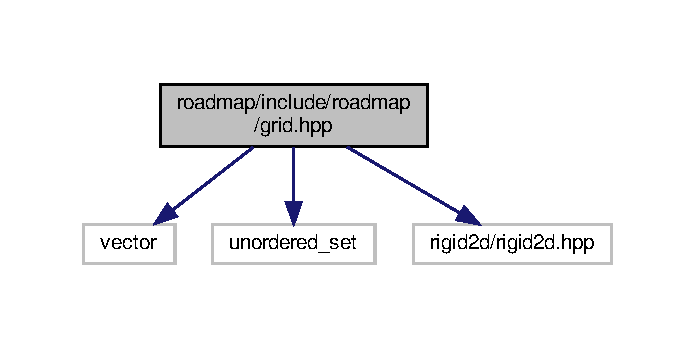
\includegraphics[width=334pt]{d7/da1/grid_8hpp__incl}
\end{center}
\end{figure}
This graph shows which files directly or indirectly include this file\+:\nopagebreak
\begin{figure}[H]
\begin{center}
\leavevmode
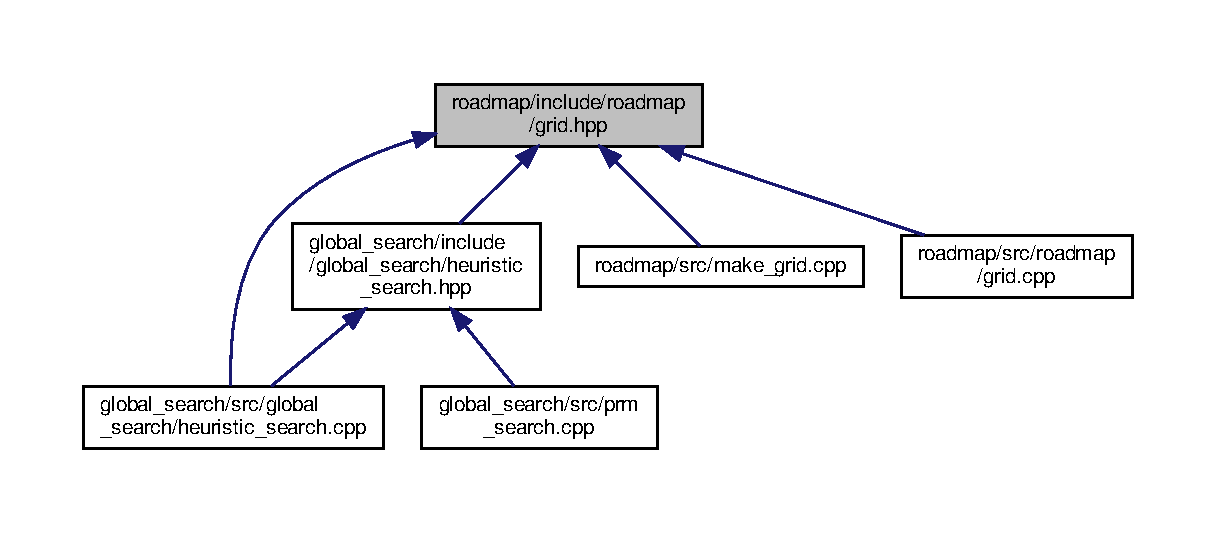
\includegraphics[width=208pt]{db/d6c/grid_8hpp__dep__incl}
\end{center}
\end{figure}
\subsection*{Classes}
\begin{DoxyCompactItemize}
\item 
struct \hyperlink{structgrid_1_1Map}{grid\+::\+Map}
\begin{DoxyCompactList}\small\item\em Contains information about a bound map. \end{DoxyCompactList}\item 
class \hyperlink{classgrid_1_1Grid}{grid\+::\+Grid}
\begin{DoxyCompactList}\small\item\em Class to create a \hyperlink{classgrid_1_1Grid}{Grid} overlay for provided \hyperlink{structgrid_1_1Map}{Map} information. \end{DoxyCompactList}\end{DoxyCompactItemize}


\subsection{Detailed Description}
A library for building an occupancy grid. 


\hypertarget{prm_8hpp}{}\section{roadmap/include/roadmap/prm.hpp File Reference}
\label{prm_8hpp}\index{roadmap/include/roadmap/prm.\+hpp@{roadmap/include/roadmap/prm.\+hpp}}


A library for building a Probabilistic Road Map.  


{\ttfamily \#include $<$vector$>$}\newline
{\ttfamily \#include $<$unordered\+\_\+set$>$}\newline
{\ttfamily \#include \char`\"{}rigid2d/rigid2d.\+hpp\char`\"{}}\newline
Include dependency graph for prm.\+hpp\+:
\nopagebreak
\begin{figure}[H]
\begin{center}
\leavevmode
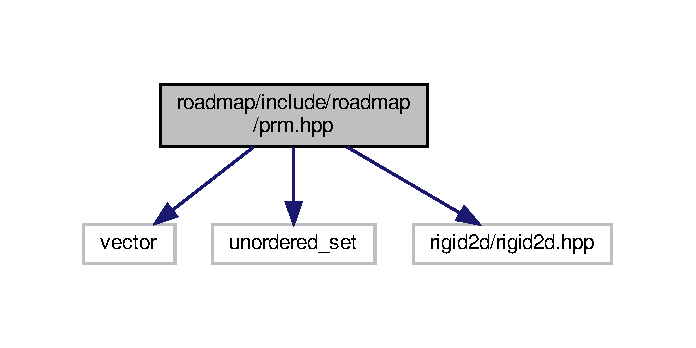
\includegraphics[width=334pt]{d7/d00/prm_8hpp__incl}
\end{center}
\end{figure}
This graph shows which files directly or indirectly include this file\+:
\nopagebreak
\begin{figure}[H]
\begin{center}
\leavevmode
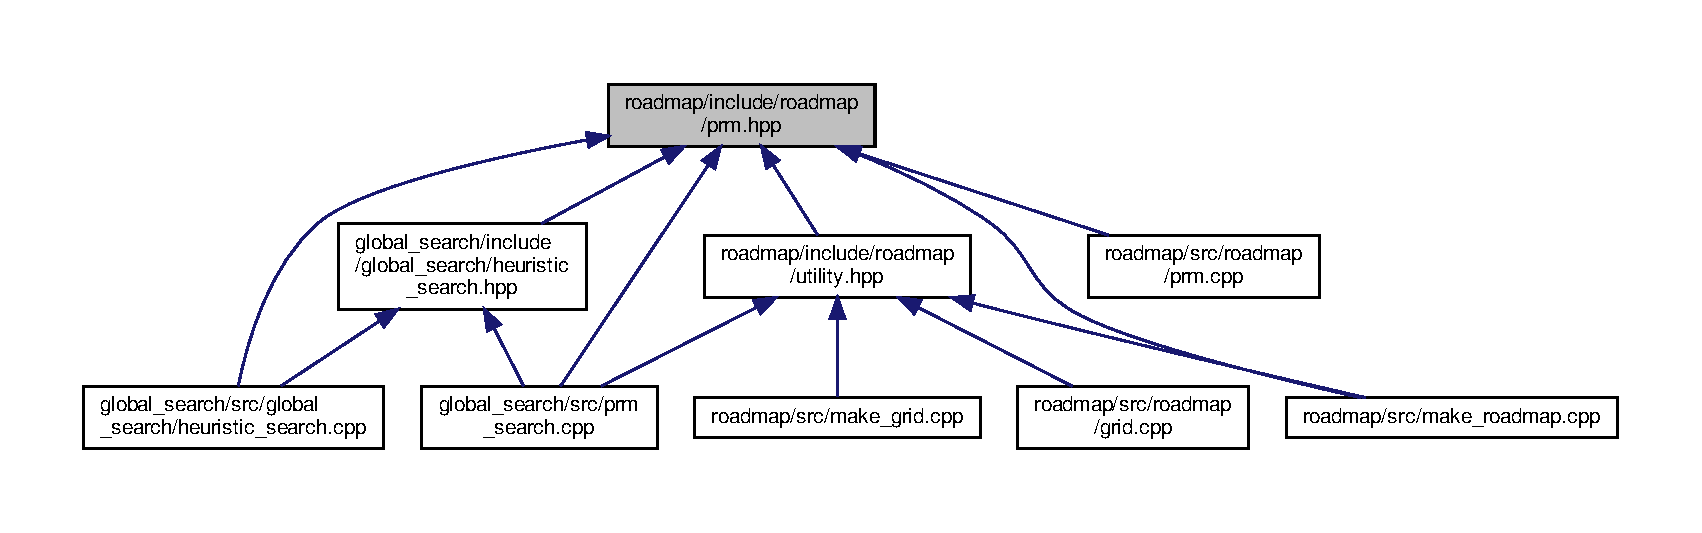
\includegraphics[width=350pt]{d6/d45/prm_8hpp__dep__incl}
\end{center}
\end{figure}
\subsection*{Classes}
\begin{DoxyCompactItemize}
\item 
struct \hyperlink{structprm_1_1Edge}{prm\+::\+Edge}
\begin{DoxyCompactList}\small\item\em A struct to fully describe a connection between two nodes. \end{DoxyCompactList}\item 
struct \hyperlink{structprm_1_1Node}{prm\+::\+Node}
\begin{DoxyCompactList}\small\item\em A struct to define a node and interact with it. \end{DoxyCompactList}\item 
class \hyperlink{classprm_1_1RoadMap}{prm\+::\+Road\+Map}
\begin{DoxyCompactList}\small\item\em A class to build a Probabilistic Road Maps based on provided Map information. \end{DoxyCompactList}\end{DoxyCompactItemize}


\subsection{Detailed Description}
A library for building a Probabilistic Road Map. 


\hypertarget{utility_8hpp}{}\section{roadmap/include/roadmap/utility.hpp File Reference}
\label{utility_8hpp}\index{roadmap/include/roadmap/utility.\+hpp@{roadmap/include/roadmap/utility.\+hpp}}


A library of utility functions for the various nodes and libraries of this package.  


{\ttfamily \#include $<$vector$>$}\newline
{\ttfamily \#include $<$Xml\+Rpc\+Value.\+h$>$}\newline
{\ttfamily \#include \char`\"{}rigid2d/rigid2d.\+hpp\char`\"{}}\newline
Include dependency graph for utility.\+hpp\+:
\nopagebreak
\begin{figure}[H]
\begin{center}
\leavevmode
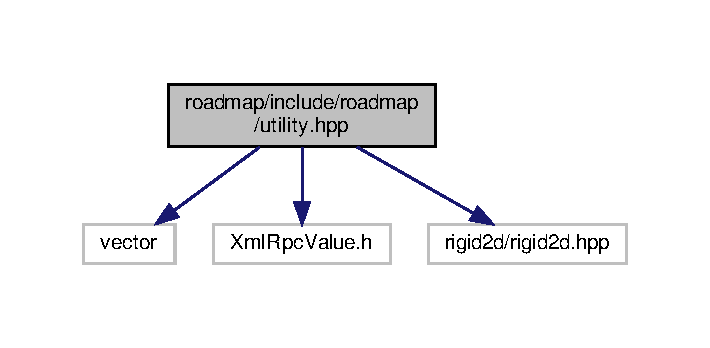
\includegraphics[width=341pt]{d1/d48/utility_8hpp__incl}
\end{center}
\end{figure}
This graph shows which files directly or indirectly include this file\+:
\nopagebreak
\begin{figure}[H]
\begin{center}
\leavevmode
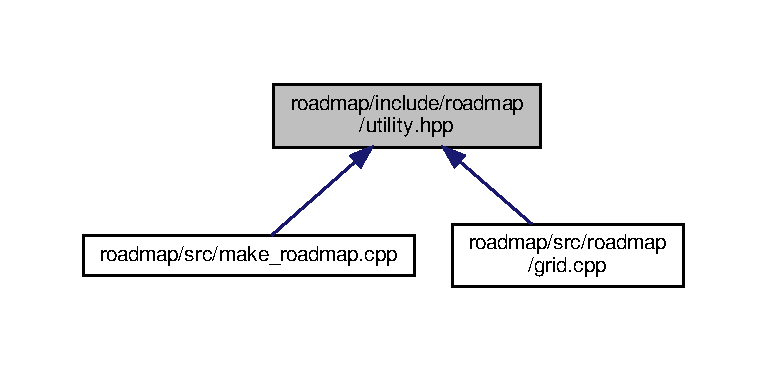
\includegraphics[width=350pt]{d7/d68/utility_8hpp__dep__incl}
\end{center}
\end{figure}
\subsection*{Functions}
\begin{DoxyCompactItemize}
\item 
std\+::vector$<$ std\+::vector$<$ rigid2d\+::\+Vector2D $>$ $>$ \hyperlink{utility_8hpp_a146978c7eb3e5b6e8604499596442f9e}{utility\+::parse\+\_\+obstacle\+\_\+data} (Xml\+Rpc\+::\+Xml\+Rpc\+Value obstacles, double cell\+\_\+size)
\begin{DoxyCompactList}\small\item\em converts obstacle data from a Y\+A\+ML file into a vector of vectors. T\+O\+DO\+: changes this to a template based output \end{DoxyCompactList}\item 
std\+::vector$<$ rigid2d\+::\+Vector2D $>$ \hyperlink{utility_8hpp_a9eb7f849405aea8fd6215f962f7d77a2}{utility\+::create\+\_\+map\+\_\+vector} (std\+::vector$<$ double $>$ map\+\_\+x\+\_\+lims, std\+::vector$<$ double $>$ map\+\_\+y\+\_\+lims)
\begin{DoxyCompactList}\small\item\em gerenate a vector of the 4 map verticies \end{DoxyCompactList}\end{DoxyCompactItemize}


\subsection{Detailed Description}
A library of utility functions for the various nodes and libraries of this package. 



\subsection{Function Documentation}
\mbox{\Hypertarget{utility_8hpp_file_a9eb7f849405aea8fd6215f962f7d77a2}\label{utility_8hpp_file_a9eb7f849405aea8fd6215f962f7d77a2}} 
\index{utility.\+hpp@{utility.\+hpp}!create\+\_\+map\+\_\+vector@{create\+\_\+map\+\_\+vector}}
\index{create\+\_\+map\+\_\+vector@{create\+\_\+map\+\_\+vector}!utility.\+hpp@{utility.\+hpp}}
\subsubsection{\texorpdfstring{create\+\_\+map\+\_\+vector()}{create\_map\_vector()}}
{\footnotesize\ttfamily std\+::vector$<$ rigid2d\+::\+Vector2D $>$ utility\+::create\+\_\+map\+\_\+vector (\begin{DoxyParamCaption}\item[{std\+::vector$<$ double $>$}]{map\+\_\+x\+\_\+lims,  }\item[{std\+::vector$<$ double $>$}]{map\+\_\+y\+\_\+lims }\end{DoxyParamCaption})}



gerenate a vector of the 4 map verticies 


\begin{DoxyParams}{Parameters}
{\em map\+\_\+x\+\_\+lims} & the x axis limits of the map \\
\hline
{\em map\+\_\+y\+\_\+lims} & the y axis limits of the map \\
\hline
\end{DoxyParams}
\begin{DoxyReturn}{Returns}
a vector of the map verticies in ccw order 
\end{DoxyReturn}
\mbox{\Hypertarget{utility_8hpp_file_a146978c7eb3e5b6e8604499596442f9e}\label{utility_8hpp_file_a146978c7eb3e5b6e8604499596442f9e}} 
\index{utility.\+hpp@{utility.\+hpp}!parse\+\_\+obstacle\+\_\+data@{parse\+\_\+obstacle\+\_\+data}}
\index{parse\+\_\+obstacle\+\_\+data@{parse\+\_\+obstacle\+\_\+data}!utility.\+hpp@{utility.\+hpp}}
\subsubsection{\texorpdfstring{parse\+\_\+obstacle\+\_\+data()}{parse\_obstacle\_data()}}
{\footnotesize\ttfamily std\+::vector$<$ std\+::vector$<$ rigid2d\+::\+Vector2D $>$ $>$ utility\+::parse\+\_\+obstacle\+\_\+data (\begin{DoxyParamCaption}\item[{Xml\+Rpc\+::\+Xml\+Rpc\+Value}]{obstacles,  }\item[{double}]{cell\+\_\+size }\end{DoxyParamCaption})}



converts obstacle data from a Y\+A\+ML file into a vector of vectors. T\+O\+DO\+: changes this to a template based output 


\begin{DoxyParams}{Parameters}
{\em obstacles} & the a list of lists containing obstacle vertices \\
\hline
{\em cell\+\_\+size} & a scaling factor to apply to the vertex coordinates. Use 1 if you do not want to scale them. \\
\hline
\end{DoxyParams}
\begin{DoxyReturn}{Returns}
a vector of vectors containing obstacle vertices 
\end{DoxyReturn}

\hypertarget{draw__world_8cpp}{}\section{roadmap/src/draw\+\_\+world.cpp File Reference}
\label{draw__world_8cpp}\index{roadmap/src/draw\+\_\+world.\+cpp@{roadmap/src/draw\+\_\+world.\+cpp}}


Node to draw the features of the real world map.  


{\ttfamily \#include $<$vector$>$}\newline
{\ttfamily \#include $<$Xml\+Rpc\+Value.\+h$>$}\newline
{\ttfamily \#include $<$ros/ros.\+h$>$}\newline
{\ttfamily \#include \char`\"{}geometry\+\_\+msgs/\+Point.\+h\char`\"{}}\newline
{\ttfamily \#include \char`\"{}visualization\+\_\+msgs/\+Marker\+Array.\+h\char`\"{}}\newline
{\ttfamily \#include \char`\"{}visualization\+\_\+msgs/\+Marker.\+h\char`\"{}}\newline
{\ttfamily \#include \char`\"{}rigid2d/rigid2d.\+hpp\char`\"{}}\newline
Include dependency graph for draw\+\_\+world.\+cpp\+:
\nopagebreak
\begin{figure}[H]
\begin{center}
\leavevmode
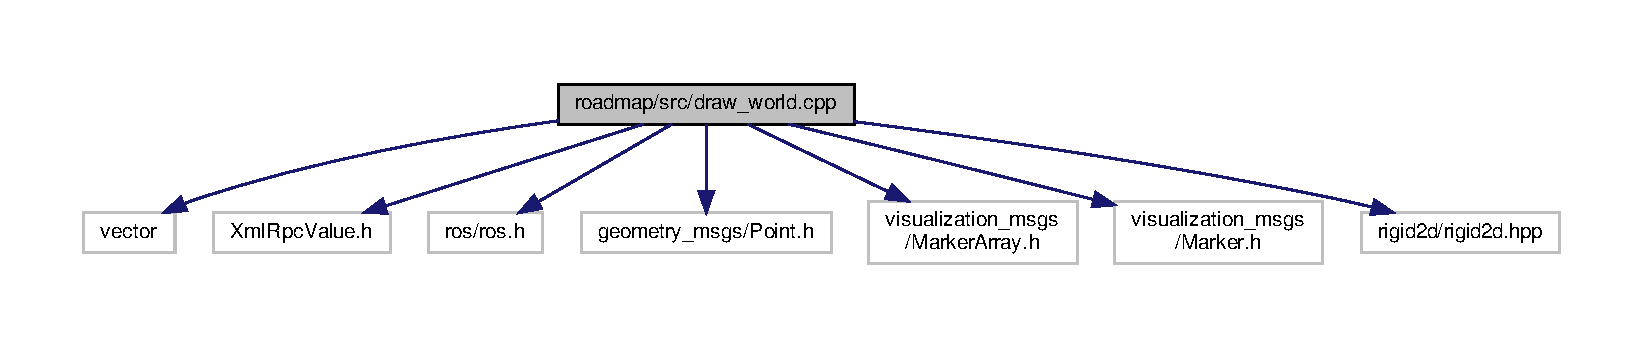
\includegraphics[width=350pt]{d2/dd7/draw__world_8cpp__incl}
\end{center}
\end{figure}
\subsection*{Functions}
\begin{DoxyCompactItemize}
\item 
\mbox{\Hypertarget{draw__world_8cpp_a3c04138a5bfe5d72780bb7e82a18e627}\label{draw__world_8cpp_a3c04138a5bfe5d72780bb7e82a18e627}} 
int {\bfseries main} (int argc, char $\ast$$\ast$argv)
\end{DoxyCompactItemize}


\subsection{Detailed Description}
Node to draw the features of the real world map. 

P\+A\+R\+A\+M\+E\+T\+E\+RS\+: obstacles (std\+::vector$<$std\+::vector$<$std\+::vector$<$double$>$) a vector of polygons represented by a vector of x,y coords for the verticies map\+\_\+x\+\_\+lims (std\+::vector$<$double$>$) \mbox{[}xmin, xmax\mbox{]} of the map map\+\_\+y\+\_\+lims (std\+::vector$<$double$>$) \mbox{[}ymin, ymax\mbox{]} of the map r (std\+::vector$<$int$>$) color values g (std\+::vector$<$int$>$) color values b (std\+::vector$<$int$>$) color values P\+U\+B\+L\+I\+S\+H\+ES\+: /visualization\+\_\+marker\+\_\+array (visualization\+\_\+msgs\+::\+Marker\+Array) markers 
\hypertarget{make__roadmap_8cpp}{}\section{roadmap/src/make\+\_\+roadmap.cpp File Reference}
\label{make__roadmap_8cpp}\index{roadmap/src/make\+\_\+roadmap.\+cpp@{roadmap/src/make\+\_\+roadmap.\+cpp}}


Node to create and draw a probabilistic road map.  


{\ttfamily \#include $<$vector$>$}\newline
{\ttfamily \#include $<$algorithm$>$}\newline
{\ttfamily \#include $<$Xml\+Rpc\+Value.\+h$>$}\newline
{\ttfamily \#include $<$ros/ros.\+h$>$}\newline
{\ttfamily \#include \char`\"{}geometry\+\_\+msgs/\+Point.\+h\char`\"{}}\newline
{\ttfamily \#include \char`\"{}visualization\+\_\+msgs/\+Marker\+Array.\+h\char`\"{}}\newline
{\ttfamily \#include \char`\"{}visualization\+\_\+msgs/\+Marker.\+h\char`\"{}}\newline
{\ttfamily \#include \char`\"{}rigid2d/rigid2d.\+hpp\char`\"{}}\newline
{\ttfamily \#include \char`\"{}roadmap/prm.\+hpp\char`\"{}}\newline
{\ttfamily \#include \char`\"{}roadmap/utility.\+hpp\char`\"{}}\newline
Include dependency graph for make\+\_\+roadmap.\+cpp\+:
\nopagebreak
\begin{figure}[H]
\begin{center}
\leavevmode
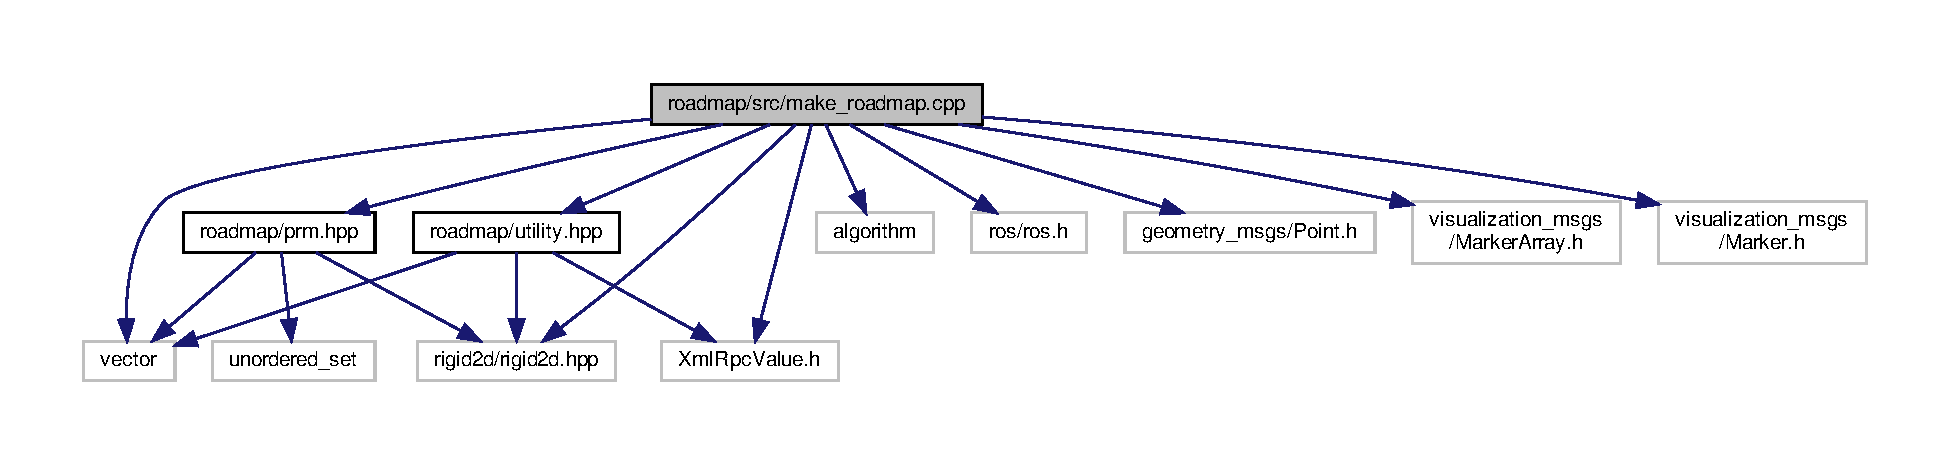
\includegraphics[width=350pt]{df/d6e/make__roadmap_8cpp__incl}
\end{center}
\end{figure}
\subsection*{Functions}
\begin{DoxyCompactItemize}
\item 
\mbox{\Hypertarget{make__roadmap_8cpp_a3c04138a5bfe5d72780bb7e82a18e627}\label{make__roadmap_8cpp_a3c04138a5bfe5d72780bb7e82a18e627}} 
int {\bfseries main} (int argc, char $\ast$$\ast$argv)
\end{DoxyCompactItemize}


\subsection{Detailed Description}
Node to create and draw a probabilistic road map. 

P\+A\+R\+A\+M\+E\+T\+E\+RS\+: obstacles (std\+::vector$<$std\+::vector$<$std\+::vector$<$double$>$) a vector of polygons represented by a vector of x,y coords for the verticies map\+\_\+x\+\_\+lims (std\+::vector$<$double$>$) \mbox{[}xmin, xmax\mbox{]} of the map map\+\_\+y\+\_\+lims (std\+::vector$<$double$>$) \mbox{[}ymin, ymax\mbox{]} of the map robot\+\_\+radius (double) buffer radius to avoid collisions with the robot body k\+\_\+nearest (unsigned int) number of neighboring verticies to match to graph\+\_\+size (unsigned int) number of nodes to use to build the graph r (std\+::vector$<$int$>$) color values g (std\+::vector$<$int$>$) color values b (std\+::vector$<$int$>$) color values P\+U\+B\+L\+I\+S\+H\+ES\+: /visualization\+\_\+marker\+\_\+array (visualization\+\_\+msgs\+::\+Marker\+Array) markers 
\hypertarget{collision_8cpp}{}\section{roadmap/src/roadmap/collision.cpp File Reference}
\label{collision_8cpp}\index{roadmap/src/roadmap/collision.\+cpp@{roadmap/src/roadmap/collision.\+cpp}}


A library containing functions to detect various types of collisions.  


{\ttfamily \#include $<$algorithm$>$}\newline
{\ttfamily \#include $<$functional$>$}\newline
{\ttfamily \#include $<$iostream$>$}\newline
{\ttfamily \#include $<$vector$>$}\newline
{\ttfamily \#include \char`\"{}roadmap/collision.\+hpp\char`\"{}}\newline
{\ttfamily \#include \char`\"{}rigid2d/rigid2d.\+hpp\char`\"{}}\newline
Include dependency graph for collision.\+cpp\+:
\nopagebreak
\begin{figure}[H]
\begin{center}
\leavevmode
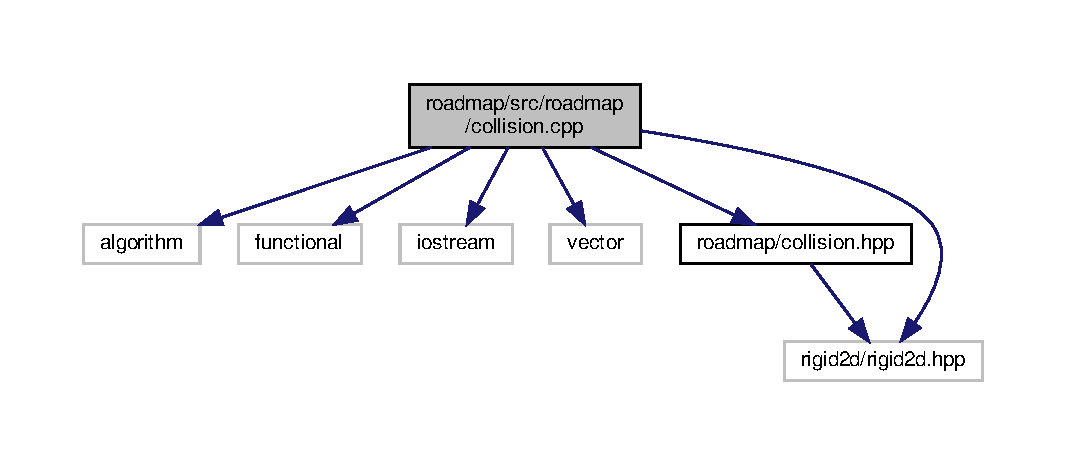
\includegraphics[width=350pt]{d9/d5a/collision_8cpp__incl}
\end{center}
\end{figure}
\subsection*{Functions}
\begin{DoxyCompactItemize}
\item 
Dist\+Res \hyperlink{collision_8hpp_a7ac784d9a63acc273489e7e61c45416a}{collision\+::point\+\_\+to\+\_\+line\+\_\+distance} (rigid2d\+::\+Vector2D line\+\_\+start, rigid2d\+::\+Vector2D line\+\_\+end, rigid2d\+::\+Vector2D point)
\begin{DoxyCompactList}\small\item\em Determine if a point is within a certain distance to a line. \end{DoxyCompactList}\item 
bool \hyperlink{collision_8hpp_aabf5aea7b02c454140c9bb242ca6e944}{collision\+::point\+\_\+to\+\_\+line\+\_\+distance} (rigid2d\+::\+Vector2D line\+\_\+start, rigid2d\+::\+Vector2D line\+\_\+end, rigid2d\+::\+Vector2D point, double threshold)
\begin{DoxyCompactList}\small\item\em Determine if a point is within a certain distance to a line. \end{DoxyCompactList}\item 
std\+::vector$<$ bool $>$ \hyperlink{collision_8hpp_af534ea532917e73ac2b28ca11c6cdf9f}{collision\+::point\+\_\+inside\+\_\+convex} (rigid2d\+::\+Vector2D point, std\+::vector$<$ rigid2d\+::\+Vector2D $>$ polygon, double buffer\+\_\+radius)
\begin{DoxyCompactList}\small\item\em Determine if a point is inside of a convex polygon, the points must be provided in order either cw or ccw. This function will account for connected the last vertex to the first vertex by appending the first vertex to the back of the vector. \end{DoxyCompactList}\item 
bool \hyperlink{collision_8hpp_a70c9083464a3dd4bc7c32dabe857e331}{collision\+::line\+\_\+shape\+\_\+intersection} (rigid2d\+::\+Vector2D line\+\_\+start, rigid2d\+::\+Vector2D line\+\_\+end, std\+::vector$<$ rigid2d\+::\+Vector2D $>$ polygon)
\begin{DoxyCompactList}\small\item\em Determine if a line segment intersects a convex polygon. \end{DoxyCompactList}\item 
bool \hyperlink{collision_8hpp_abf9b390bd1d767fe39f7d4806fae6b62}{collision\+::line\+\_\+shape\+\_\+intersection} (rigid2d\+::\+Vector2D line\+\_\+start, rigid2d\+::\+Vector2D line\+\_\+end, std\+::vector$<$ rigid2d\+::\+Vector2D $>$ polygon, double buffer\+\_\+radius)
\begin{DoxyCompactList}\small\item\em Determine if a line segment intersects a convex polygon or comes within a certain distance of it. This assumes the line start and end points are known to be outside of the buffer area of the polygon. \end{DoxyCompactList}\end{DoxyCompactItemize}


\subsection{Detailed Description}
A library containing functions to detect various types of collisions. 



\subsection{Function Documentation}
\mbox{\Hypertarget{collision_8hpp_file_a70c9083464a3dd4bc7c32dabe857e331}\label{collision_8hpp_file_a70c9083464a3dd4bc7c32dabe857e331}} 
\index{collision.\+cpp@{collision.\+cpp}!line\+\_\+shape\+\_\+intersection@{line\+\_\+shape\+\_\+intersection}}
\index{line\+\_\+shape\+\_\+intersection@{line\+\_\+shape\+\_\+intersection}!collision.\+cpp@{collision.\+cpp}}
\subsubsection{\texorpdfstring{line\+\_\+shape\+\_\+intersection()}{line\_shape\_intersection()}\hspace{0.1cm}{\footnotesize\ttfamily [1/2]}}
{\footnotesize\ttfamily bool collision\+::line\+\_\+shape\+\_\+intersection (\begin{DoxyParamCaption}\item[{rigid2d\+::\+Vector2D}]{line\+\_\+start,  }\item[{rigid2d\+::\+Vector2D}]{line\+\_\+end,  }\item[{std\+::vector$<$ rigid2d\+::\+Vector2D $>$}]{polygon }\end{DoxyParamCaption})}



Determine if a line segment intersects a convex polygon. 


\begin{DoxyParams}{Parameters}
{\em line\+\_\+start} & the point of the beginning of the line segment \\
\hline
{\em line\+\_\+end} & the point of the end of the line segment \\
\hline
{\em polygon} & a vector of verticies that define the polygon in ccw order \\
\hline
\end{DoxyParams}
\begin{DoxyReturn}{Returns}
True if there is an intersection between the line segment and polygon 
\end{DoxyReturn}
\mbox{\Hypertarget{collision_8hpp_file_abf9b390bd1d767fe39f7d4806fae6b62}\label{collision_8hpp_file_abf9b390bd1d767fe39f7d4806fae6b62}} 
\index{collision.\+cpp@{collision.\+cpp}!line\+\_\+shape\+\_\+intersection@{line\+\_\+shape\+\_\+intersection}}
\index{line\+\_\+shape\+\_\+intersection@{line\+\_\+shape\+\_\+intersection}!collision.\+cpp@{collision.\+cpp}}
\subsubsection{\texorpdfstring{line\+\_\+shape\+\_\+intersection()}{line\_shape\_intersection()}\hspace{0.1cm}{\footnotesize\ttfamily [2/2]}}
{\footnotesize\ttfamily bool collision\+::line\+\_\+shape\+\_\+intersection (\begin{DoxyParamCaption}\item[{rigid2d\+::\+Vector2D}]{line\+\_\+start,  }\item[{rigid2d\+::\+Vector2D}]{line\+\_\+end,  }\item[{std\+::vector$<$ rigid2d\+::\+Vector2D $>$}]{polygon,  }\item[{double}]{buffer\+\_\+radius }\end{DoxyParamCaption})}



Determine if a line segment intersects a convex polygon or comes within a certain distance of it. This assumes the line start and end points are known to be outside of the buffer area of the polygon. 


\begin{DoxyParams}{Parameters}
{\em line\+\_\+start} & the point of the beginning of the line segment \\
\hline
{\em line\+\_\+end} & the point of the end of the line segment \\
\hline
{\em polygon} & a vector of verticies that define the polygon in ccw order \\
\hline
{\em buffer\+\_\+radius} & a buffer distance to incorporate to the polygon boundary \\
\hline
\end{DoxyParams}
\begin{DoxyReturn}{Returns}
True if there is an intersection between the line segment and polygon or if the minimum distance to the line and shape is less than the buffer radius 
\end{DoxyReturn}
\mbox{\Hypertarget{collision_8hpp_file_af534ea532917e73ac2b28ca11c6cdf9f}\label{collision_8hpp_file_af534ea532917e73ac2b28ca11c6cdf9f}} 
\index{collision.\+cpp@{collision.\+cpp}!point\+\_\+inside\+\_\+convex@{point\+\_\+inside\+\_\+convex}}
\index{point\+\_\+inside\+\_\+convex@{point\+\_\+inside\+\_\+convex}!collision.\+cpp@{collision.\+cpp}}
\subsubsection{\texorpdfstring{point\+\_\+inside\+\_\+convex()}{point\_inside\_convex()}}
{\footnotesize\ttfamily std\+::vector$<$ bool $>$ collision\+::point\+\_\+inside\+\_\+convex (\begin{DoxyParamCaption}\item[{rigid2d\+::\+Vector2D}]{point,  }\item[{std\+::vector$<$ rigid2d\+::\+Vector2D $>$}]{polygon,  }\item[{double}]{buffer\+\_\+radius }\end{DoxyParamCaption})}



Determine if a point is inside of a convex polygon, the points must be provided in order either cw or ccw. This function will account for connected the last vertex to the first vertex by appending the first vertex to the back of the vector. 


\begin{DoxyParams}{Parameters}
{\em point} & the point to analyze \\
\hline
{\em polygon} & a vector of verticies that define the polygon in order, either cw or ccw. \\
\hline
{\em buffer\+\_\+radius} & a buffer distance to incorporate to the polygon boundary \\
\hline
\end{DoxyParams}
\begin{DoxyReturn}{Returns}
a 2 element vector, first element is true if there is a collision, second element describes the cause\+: True for inside the shape, False for outside the shape, but in the buffer zone. 
\end{DoxyReturn}
\mbox{\Hypertarget{collision_8hpp_file_aabf5aea7b02c454140c9bb242ca6e944}\label{collision_8hpp_file_aabf5aea7b02c454140c9bb242ca6e944}} 
\index{collision.\+cpp@{collision.\+cpp}!point\+\_\+to\+\_\+line\+\_\+distance@{point\+\_\+to\+\_\+line\+\_\+distance}}
\index{point\+\_\+to\+\_\+line\+\_\+distance@{point\+\_\+to\+\_\+line\+\_\+distance}!collision.\+cpp@{collision.\+cpp}}
\subsubsection{\texorpdfstring{point\+\_\+to\+\_\+line\+\_\+distance()}{point\_to\_line\_distance()}\hspace{0.1cm}{\footnotesize\ttfamily [1/2]}}
{\footnotesize\ttfamily bool collision\+::point\+\_\+to\+\_\+line\+\_\+distance (\begin{DoxyParamCaption}\item[{rigid2d\+::\+Vector2D}]{line\+\_\+start,  }\item[{rigid2d\+::\+Vector2D}]{line\+\_\+end,  }\item[{rigid2d\+::\+Vector2D}]{point,  }\item[{double}]{threshold }\end{DoxyParamCaption})}



Determine if a point is within a certain distance to a line. 


\begin{DoxyParams}{Parameters}
{\em line\+\_\+start} & the point of the beginning of the line segment \\
\hline
{\em line\+\_\+end} & the point of the end of the line segment \\
\hline
{\em point} & the point to calculate the distance for \\
\hline
{\em threshold} & the distance threshold to compare against \\
\hline
\end{DoxyParams}
\begin{DoxyReturn}{Returns}
True if the distance between the point and the line is L\+E\+SS T\+H\+AN the provided threshold 
\end{DoxyReturn}
\mbox{\Hypertarget{collision_8hpp_file_a7ac784d9a63acc273489e7e61c45416a}\label{collision_8hpp_file_a7ac784d9a63acc273489e7e61c45416a}} 
\index{collision.\+cpp@{collision.\+cpp}!point\+\_\+to\+\_\+line\+\_\+distance@{point\+\_\+to\+\_\+line\+\_\+distance}}
\index{point\+\_\+to\+\_\+line\+\_\+distance@{point\+\_\+to\+\_\+line\+\_\+distance}!collision.\+cpp@{collision.\+cpp}}
\subsubsection{\texorpdfstring{point\+\_\+to\+\_\+line\+\_\+distance()}{point\_to\_line\_distance()}\hspace{0.1cm}{\footnotesize\ttfamily [2/2]}}
{\footnotesize\ttfamily Dist\+Res collision\+::point\+\_\+to\+\_\+line\+\_\+distance (\begin{DoxyParamCaption}\item[{rigid2d\+::\+Vector2D}]{line\+\_\+start,  }\item[{rigid2d\+::\+Vector2D}]{line\+\_\+end,  }\item[{rigid2d\+::\+Vector2D}]{point }\end{DoxyParamCaption})}



Determine if a point is within a certain distance to a line. 


\begin{DoxyParams}{Parameters}
{\em line\+\_\+start} & the point of the beginning of the line segment \\
\hline
{\em line\+\_\+end} & the point of the end of the line segment \\
\hline
{\em point} & the point to calculate the distance for \\
\hline
\end{DoxyParams}
\begin{DoxyReturn}{Returns}
The shortest distance between the point and the line if the point is within the line segment or the minimum between the distances to the line\+\_\+start or line\+\_\+end 
\end{DoxyReturn}

\hypertarget{grid_8cpp}{}\section{roadmap/src/roadmap/grid.cpp File Reference}
\label{grid_8cpp}\index{roadmap/src/roadmap/grid.\+cpp@{roadmap/src/roadmap/grid.\+cpp}}


A library for building an occupied grid.  


{\ttfamily \#include $<$algorithm$>$}\newline
{\ttfamily \#include $<$functional$>$}\newline
{\ttfamily \#include $<$iostream$>$}\newline
{\ttfamily \#include $<$random$>$}\newline
{\ttfamily \#include $<$unordered\+\_\+set$>$}\newline
{\ttfamily \#include $<$vector$>$}\newline
{\ttfamily \#include \char`\"{}roadmap/collision.\+hpp\char`\"{}}\newline
{\ttfamily \#include \char`\"{}roadmap/grid.\+hpp\char`\"{}}\newline
{\ttfamily \#include \char`\"{}roadmap/utility.\+hpp\char`\"{}}\newline
{\ttfamily \#include \char`\"{}rigid2d/rigid2d.\+hpp\char`\"{}}\newline
Include dependency graph for grid.\+cpp\+:
\nopagebreak
\begin{figure}[H]
\begin{center}
\leavevmode
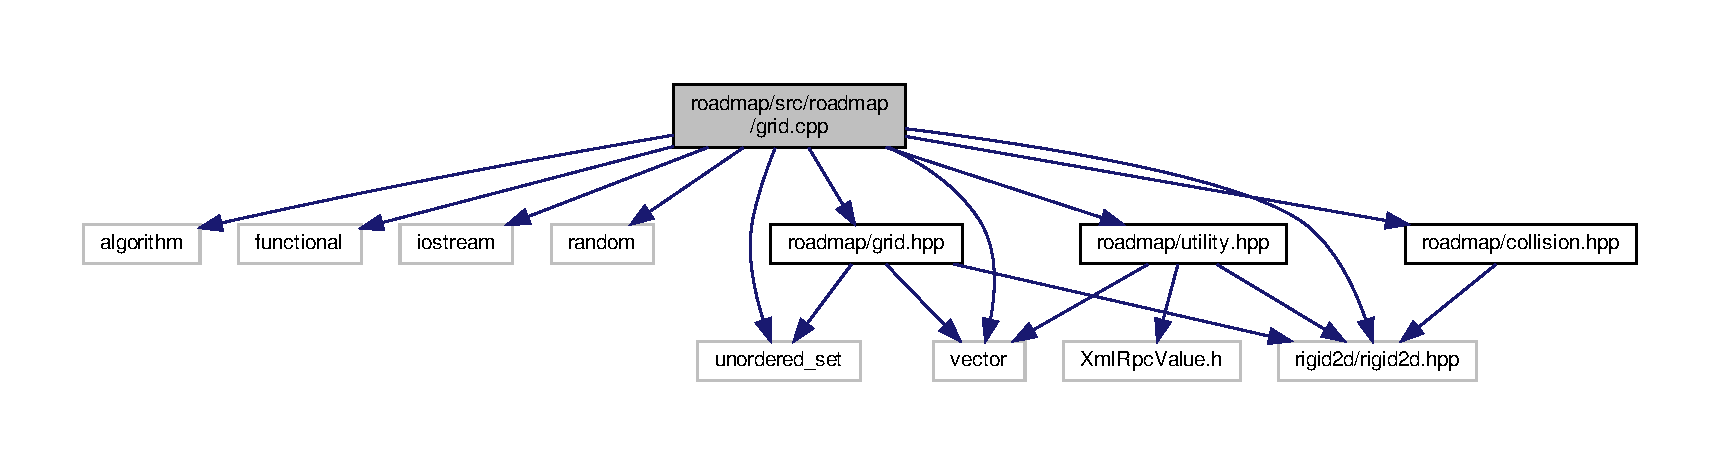
\includegraphics[width=350pt]{da/d1e/grid_8cpp__incl}
\end{center}
\end{figure}


\subsection{Detailed Description}
A library for building an occupied grid. 


\hypertarget{prm_8cpp}{}\section{roadmap/src/roadmap/prm.cpp File Reference}
\label{prm_8cpp}\index{roadmap/src/roadmap/prm.\+cpp@{roadmap/src/roadmap/prm.\+cpp}}


A library for building a Probabilistic Road Map.  


{\ttfamily \#include $<$algorithm$>$}\newline
{\ttfamily \#include $<$functional$>$}\newline
{\ttfamily \#include $<$iostream$>$}\newline
{\ttfamily \#include $<$random$>$}\newline
{\ttfamily \#include $<$unordered\+\_\+set$>$}\newline
{\ttfamily \#include $<$vector$>$}\newline
{\ttfamily \#include \char`\"{}roadmap/prm.\+hpp\char`\"{}}\newline
{\ttfamily \#include \char`\"{}roadmap/collision.\+hpp\char`\"{}}\newline
{\ttfamily \#include \char`\"{}rigid2d/rigid2d.\+hpp\char`\"{}}\newline
Include dependency graph for prm.\+cpp\+:
\nopagebreak
\begin{figure}[H]
\begin{center}
\leavevmode
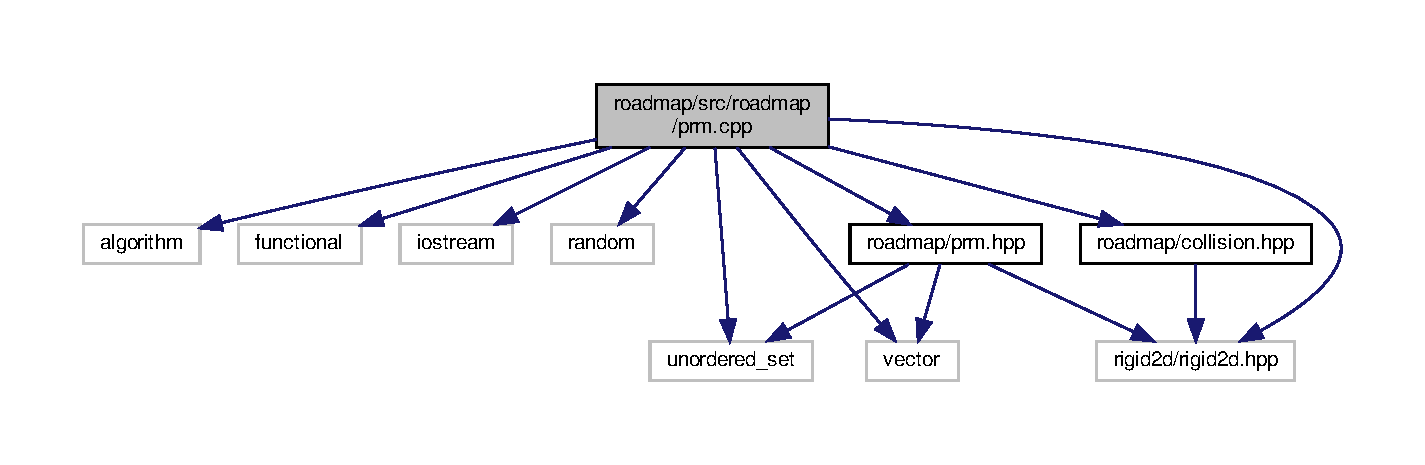
\includegraphics[width=350pt]{d9/d55/prm_8cpp__incl}
\end{center}
\end{figure}
\subsection*{Functions}
\begin{DoxyCompactItemize}
\item 
double \hyperlink{prm_8cpp_a88d1f8babd798649cc2fe9a223e48778}{prm\+::sample\+Uniform\+Distribution} (double llim, double ulim)
\begin{DoxyCompactList}\small\item\em Sample a random value between the provided limits. \end{DoxyCompactList}\end{DoxyCompactItemize}


\subsection{Detailed Description}
A library for building a Probabilistic Road Map. 



\subsection{Function Documentation}
\mbox{\Hypertarget{prm_8cpp_file_a88d1f8babd798649cc2fe9a223e48778}\label{prm_8cpp_file_a88d1f8babd798649cc2fe9a223e48778}} 
\index{prm.\+cpp@{prm.\+cpp}!sample\+Uniform\+Distribution@{sample\+Uniform\+Distribution}}
\index{sample\+Uniform\+Distribution@{sample\+Uniform\+Distribution}!prm.\+cpp@{prm.\+cpp}}
\subsubsection{\texorpdfstring{sample\+Uniform\+Distribution()}{sampleUniformDistribution()}}
{\footnotesize\ttfamily double prm\+::sample\+Uniform\+Distribution (\begin{DoxyParamCaption}\item[{double}]{llim,  }\item[{double}]{ulim }\end{DoxyParamCaption})}



Sample a random value between the provided limits. 


\begin{DoxyParams}{Parameters}
{\em llim} & the lower bound of the range \\
\hline
{\em ulim} & the upper bound of the range \\
\hline
\end{DoxyParams}
\begin{DoxyReturn}{Returns}
a random value 
\end{DoxyReturn}

%--- End generated contents ---

% Index
\backmatter
\newpage
\phantomsection
\clearemptydoublepage
\addcontentsline{toc}{chapter}{Index}
\printindex

\end{document}
